\documentclass[lettersize,journal]{IEEEtran}

\usepackage{amsmath,amsfonts,amssymb}
\usepackage{algorithmic}
\usepackage{array}
\usepackage{textcomp}
\usepackage{stfloats}
\usepackage{url}
\usepackage{verbatim}
\usepackage{graphicx}
\usepackage{cite}
\usepackage{balance}
\newtheorem{theorem}{Theorem}
\newtheorem{proposition}{Proposition}
\newtheorem{lemma}{Lemma}
\newtheorem{corollary}{Corollary}
\newtheorem{remark}{Remark}
\newtheorem{assumption}{Assumption}
\hyphenation{op-tical net-works semi-conduc-tor IEEE-Xplore}
\def\BibTeX{{\rm B\kern-.05em{\sc i\kern-.025em b}\kern-.08em
    T\kern-.1667em\lower.7ex\hbox{E}\kern-.125emX}}

\urlstyle{same}
\begin{document}

\title{Multirobot Tracking of Separatrices and
Objective Eulerian Coherent Structures}

\author{Christopher Waight and Christopher A. Kitts,~\IEEEmembership{Senior Member,~IEEE}
\thanks{C. Waight is a PhD Candidate in the Robotic Systems Laboratory, Department of Mechanical Engineering, Santa Clara University, Santa Clara, CA 95053 USA (e-mail: cwaight@scu.edu)}
\thanks{C. A. Kitts is Professor and Director of the Robotic Systems Laboratory, Department of Mechanical Engineering, Santa Clara University, Santa Clara, CA 95053 USA (e-mail: ckitts@scu.edu)}
}
\markboth{IEEE Transactions on Robotics}%
{Waight and Kitts: Multirobot Tracking of Separatrices and Objective Eulerian Coherent Structures}

\maketitle

\begin{abstract}
Short-term transport in a geophysical flow is organized by
instantaneous coherent structures: curves of strongest local attraction
and repulsion, where drifting material collects within hours. Existing
robotic trackers either commit to a presumed structure in advance or
must integrate measurements over a time horizon before an estimate
exists. This paper presents a multirobot method for finding and
following these structures in real time, using only the flow velocity
each robot measures at its own position. A cooperative estimator
recovers the local quadratic model of the field from one synchronous
measurement set, and six robots are proved to be the minimum team for
this recovery under the unconstrained quadratic model. The fit supplies two trackable surrogates. The first is the Jacobian
determinant, whose valley lines trace the flow's separatrices; it is
Galilean invariant but not objective, shifting under a rotating observer.
The second is the smaller rate-of-strain eigenvalue, whose trench is
objective, a material curve recovered identically in any observer frame.
An adaptive navigation controller rides each. A rotating-frame experiment
separates them: the strain tracker's inertial and rotating runs end
0.025 apart, while the determinant tracker's diverge by 1.219 as its
rotating-frame run leaves the structure. This objectivity has a
measurable cost in robustness. Monte Carlo sweeps place the determinant
tracker's failure cliff at the estimator's own noise threshold,
$\sigma_{uv} \approx 0.01$, and the strain tracker's earlier, at
$\sigma_{uv} \approx 0.002$; at zero noise their tracking errors are
0.0016 and 0.0075. On Santa Barbara Channel radar currents, the
determinant tracker follows a coherent ridge for 28 hours to a consistent
landfall, and the strain tracker, started on that same ridge, rides the
same network structure from the objective strain term alone.
\end{abstract}

\begin{IEEEkeywords}
Multirobot Systems, Adaptive Navigation, Coherent Structures,
Okubo-Weiss, Rate of Strain, Objectivity, Cooperative
Estimation, Cluster Space Control
\end{IEEEkeywords}

\section{Introduction}
\label{sec:intro}

\IEEEPARstart{M}{ultirobot} systems build in redundancy against
individual failures, widen the area a team can cover, and spread
sensing across space rather than concentrating it at a single
platform. These systems now operate across domains from warehousing
to search and rescue \cite{1}. Equipped with field sensors, such
teams form mobile sensor networks that turn spatial spread into
simultaneous measurements at separated points.

Survey-oriented navigation puts this spatial spread to work by
sweeping a region exhaustively and identifying features only
afterward. Adaptive navigation (AN) techniques instead use
measurements in real time to drive the network toward or along
features of interest, locating local features quickly and following
them as they evolve.

AN in scalar fields is well developed. Each robot contributes a single
scalar measurement to a navigation policy that reaches and follows
features such as extrema, contour lines, ridges, trenches, saddle
points, and fronts \cite{26,27,28,29}, with formations sized so that
differential measurements across the cluster recover the gradient and
curvature each policy consumes \cite{15,26}.

Some environments are better modeled by vector fields. These models
assign both a magnitude and a direction to each point. The critical
points of that vector field often mark the features a mission cares
about, for example, in ocean currents and other geophysical flows. A
sink, for instance, can flag an area of high probability for search
and rescue, while a spewing vortex can point to a below-surface leak.
In \cite{14}, a three-robot cluster estimated the location and type of
an isolated critical point from a linear fit of simultaneous local
velocity measurements, recovering the feature from instantaneous data
alone rather than from an accumulated survey.

Beyond isolated points, there is also utility in tracking extended
features such as fronts, dynamically meaningful lines along which
water masses converge. Coordinated multi-vehicle sampling of such
dynamic ocean features is itself an active area of marine robotics,
spanning drifter-referenced AUV surveys \cite{2}, front-tracking
ASV/AUV teams \cite{3}, and adaptive glider fleets \cite{4}.

Another line of great interest is the separatrix. In steady
two-dimensional flows it is the union of the stable and unstable
manifolds through the saddle points, partitioning the domain into
basins whose trajectories do not mix. Tracking it is relevant to
dispersion modeling, pollutant containment, and coastal sensor
deployment \cite{6,7,8}, and, like the related Okubo-Weiss field used
to classify oceanic mesoscale eddies \cite{5}, it can in principle be
inferred from instantaneous measurements alone.

A line of work on separatrix navigation has equipped robot teams to
track a coherent structure directly in the flow rather than
reconstruct it offline, by straddling a presumed manifold with a small
formation \cite{9,10,11,12} or by accumulating an onboard FTLE
estimate over a finite time horizon \cite{13}. Each approach either
commits to the structure's identity before tracking begins or pays an
integration latency before an estimate exists
(Section~\ref{sec:related_robots}).

This paper's approach requires neither pre-straddling an assumed
manifold nor accumulation of data points. From an arbitrary six-robot
configuration, the team infers a structure's location, its type, and,
at a crossing, which branch to continue onto, from the current
instantaneous measurement alone. The technique exploits the fact that
the velocity gradient splits uniquely into strain plus spin,
$\mathbf{J} = \mathbf{S} + \mathbf{W}$, and that for incompressible
planar flow the determinant splits with it, $D = \omega^2/4 - s_1^2$,
where $\omega$ is the vorticity carried by $\mathbf{W}$ and $s_1$ the
smaller eigenvalue of $\mathbf{S}$ (Section~\ref{sec:detj_field}).
Each term is a trackable surrogate of the flow's transport skeleton, 
and each controller developed here rides one of them. The former surrogate 
is Galilean invariant while the latter is objective.

This paper makes four contributions. First, it presents a cooperative
second-order estimator that recovers the local quadratic model of a
two-component field from one synchronous sample, with six robots proved
minimal for the unconstrained quadratic model and with exact,
heading-isotropic noise gains. Second, it
develops the $D$ tracker, a hybrid controller built on a modified
Newton step that snaps onto a trench of $D$, slides along it, and
traverses the network of saddle crossings without committing to a
manifold identity in advance (unlike \cite{9,10}), with terminal
capture available by tightening one threshold. Third, it develops the
$s_1$ tracker, an objective controller built from the strain
eigenframe whose design follows from the structural result that no
quadratic velocity fit can certify $s_1$-trench curvature; on the
double gyre it captures reliably at a terminal core rather than
continuing past it, resolving both the attracting/repelling eigenvector
swap and the network crossing itself from objective quantities alone,
and on a field without a stationary point close enough to trigger that
capture it instead traverses the ridge network the strain term itself
resolves. Fourth, it validates both trackers under a fully specified
noise model, in a closed-loop rotating-frame objectivity experiment,
and on real Santa Barbara Channel radar currents
(Section~\ref{sec:future}).

The remainder of the paper is organized as follows. The rest of this
section reviews related work. Section~\ref{sec:detj_field} formulates
the problem. Section~\ref{sec:estimation} develops the six-robot
estimator and its accuracy under noise. Section~\ref{sec:controllers}
presents the two controllers and their stability properties, with
proofs in Appendix~\ref{app:proofs}. Section~\ref{sec:methods}
describes the simulation program and test plan, and
Section~\ref{sec:results} presents results, including the ocean
experiments. Section~\ref{sec:discussion} discusses implications and
limitations, and Section~\ref{sec:conclusion} concludes.

\subsection{Related Work}
\label{sec:related_robots}

Haller and Yuan formalized the Lagrangian coherent structure (LCS) as
the generalization of stable and unstable manifolds to flows with
arbitrary time dependence \cite{6}. The standard computable definition,
a ridge of the finite-time Lyapunov exponent (FTLE) field, is given in
\cite{8} on the same double-gyre model used throughout this paper, and
the objectivity and Lagrangian/Eulerian tradeoff that motivate this
paper's two surrogates are developed in Section~\ref{sec:detj_field},
with the underlying theory in \cite{16,17,18}. Velocity-gradient
recovery from sparse trajectories \cite{19} and the strain-spin
decomposition itself \cite{20} remain active adjacent directions. The
instantaneous criteria remain the computable workhorses: Okubo and Weiss
partition a planar flow from the local velocity gradient alone
\cite{21,22}, generalized to three dimensions \cite{23}, refined for
oceanographic use \cite{24}, and used at scale in mesoscale eddy censuses
\cite{5}.

The nearest prior work tracks a coherent structure directly with a
robot formation. Michini et al. bracket a presumed stable or unstable
manifold with three robots using only local velocity measurements
\cite{9}; the strategy extends to $N$ robots \cite{10}, was validated
on micro surface vehicles in a flow tank \cite{11}, and related
flow-based control operates marine robots in gyre-like environments
\cite{12}. Unlike methods that sense only a scalar reduction of the
field \cite{25}, the team here fits the full local quadratic vector
field, so the surrogate's shape, not merely its sign, is available to
the controllers. The straddle family commits to the manifold's identity
before tracking begins, and neither controller nor proof addresses the
saddle point itself, exactly where that identity becomes ambiguous.
Kularatne and Hsieh instead compute the local FTLE field on board,
recovering the structure's type at the price of a nonzero integration
horizon \cite{13}. None of these strategies estimates the curvature of
the field itself, which is what fixes not just where a structure lies
but what kind it is and how many branches meet there.

On the estimation side, \"{O}gren, Fiorelli, and Leonard established
cooperative gradient climbing with a formation of mobile sensors
\cite{26}, and Bri\~{n}\'{o}n-Arranz, Renzaglia, and Schenato extended
the idea to the Hessian: five robots on a ring plus one at the center
recover the gradient and Hessian of a scalar signal in closed form
\cite{15}. McDonald, Kitts, and Neumann developed the complementary
adaptive-navigation primitives that follow scalar-field ridges,
trenches, and saddle points from local differences alone
\cite{27,28,29}. Every prior formation samples one signal channel; a
coupled two-component field doubles the estimation problem to twelve
unknowns, and Section~\ref{sec:estimation} proves six robots, the same
count as the ring-plus-center of \cite{15}, is the exact minimum for
the coupled case, for any non-conic placement and against any
algorithm. Where \cite{15} inverts the raw Hessian, the modified Newton
step used here combines per-eigendirection saturation with the
saddle-free sign flip of Dauphin et al. \cite{35}, previously unapplied
to a robot team tracking a spatial field.

Robotic work in vector-field environments divides by whether the field
is measured or constructed. The critical-point and structure-tracking
methods above \cite{9,10,11,12,13,14} navigate a naturally occurring
flow that the team senses in situ. A separate and larger literature
instead builds an artificial vector field as a control law, whose
integral curves are designed to guide a single robot along a desired
path \cite{37} or around obstacles \cite{38}; there the field is a
synthetic guidance signal, not a measured environment. This paper is of
the first kind: the flow is given by the ocean, sampled locally, and its
transport skeleton is what the team is asked to find and follow.

\section{Problem Formulation}
\label{sec:detj_field}

\subsection{Vector Fields and Local Polynomial Models}

A planar vector field assigns a velocity vector $\mathbf{v}(\mathbf{p}) =
(u(\mathbf{p}), v(\mathbf{p}))$ to each position $\mathbf{p} = (x, y)$ in its
domain. The critical-point estimator of \cite{14} fits a \emph{planar}
(affine) model of each component to simultaneous measurements and solves
the linear system for the point where $\mathbf{v} = \mathbf{0}$. The
surrogates this paper tracks are built not from $\mathbf{v}$ but from its
spatial derivatives, and navigating them requires derivatives through
second order; a planar fit, whose second derivatives are identically zero,
cannot supply them.

The team therefore works from the second-order Taylor expansion of each
component about the cluster centroid $\mathbf{p}_c$. Writing
$\mathbf{p}' = (x', y') = \mathbf{p} - \mathbf{p}_c$ for position relative
to the centroid,
\begin{align}
    u(\mathbf{p}) &= u_0 + u_x x' + u_y y'
        + \tfrac{1}{2} u_{xx} {x'}^2 + u_{xy} x' y'
        + \tfrac{1}{2} u_{yy} {y'}^2
        + \mathcal{O}(\|\mathbf{p}'\|^3),
        \label{eq:quad_model_u} \\
    v(\mathbf{p}) &= v_0 + v_x x' + v_y y'
        + \tfrac{1}{2} v_{xx} {x'}^2 + v_{xy} x' y'
        + \tfrac{1}{2} v_{yy} {y'}^2
        + \mathcal{O}(\|\mathbf{p}'\|^3).
        \label{eq:quad_model_v}
\end{align}
Throughout, a subscript $0$ marks evaluation at the centroid and a
coordinate subscript marks partial differentiation, so that
$u_0 = u(\mathbf{p}_c)$, $u_x = \partial u/\partial x |_{\mathbf{p}_c}$,
and $u_{xy} = \partial^2 u/\partial x \partial y |_{\mathbf{p}_c}$. All
twelve coefficients are constants; the position dependence in
(\ref{eq:quad_model_u})--(\ref{eq:quad_model_v}) is carried entirely by
$\mathbf{p}'$.

The team estimates these coefficients by fitting the quadratic model that
remains when the $\mathcal{O}(\|\mathbf{p}'\|^3)$ remainder is discarded,
and marks the results with a hat: $\hat{u}_{xx}$ is an estimate of
$u_{xx}$, not the quantity itself. Two mechanisms separate them. Sensor
noise perturbs each measurement, and truncation bias arises because the
discarded cubic terms are not zero over a footprint of finite size, so the
fit absorbs part of them into the retained coefficients.
Section~\ref{sec:sensitivity} treats both.

The first-order coefficients are the centroid values of the entries of the
field Jacobian
\begin{equation}
    \mathbf{J}(\mathbf{p}) =
    \begin{bmatrix}
        \partial u / \partial x & \partial u / \partial y \\
        \partial v / \partial x & \partial v / \partial y
    \end{bmatrix},
    \label{eq:jacobian}
\end{equation}
so that $\mathbf{J}_0$ has entries $u_x$, $u_y$, $v_x$, $v_y$, and we write
$D(\mathbf{p}) = \det(\mathbf{J}(\mathbf{p}))$ throughout.

\subsection{Separatrices and Eulerian Surrogates}
\label{sec:separatrix}

In time-dependent flows the separatrix generalizes to LCSs, ridges of
the FTLE field \cite{6,7,8}, but computing FTLE requires integrating
dense trajectory grids over a finite horizon, exactly the global,
forward-in-time knowledge this paper's sensing model excludes. The
alternative is an Eulerian surrogate: a quantity computed pointwise
from the instantaneous field and its spatial derivatives. This paper
tracks two, both delivered by the same fit: the determinant field $D$,
Galilean invariant and globally connected, which coincides exactly with
the separatrix for the steady double gyre
(Section~\ref{sec:dg_example}); and the strain eigenvalue $s_1$, whose
trench is the objective, fully frame-invariant surrogate underlying the
attracting Eulerian coherent structures of \cite{17,18}.

\subsection{Surrogate I: the Okubo-Weiss Field $D$}

The Okubo-Weiss parameter \cite{21,22}, built from the normal strain,
shear strain, and vorticity
($\omega = \partial v/\partial x - \partial u/\partial y$), satisfies
$Q = \tfrac{1}{4}(\nabla \cdot \mathbf{v})^2 - D$ by direct expansion;
for the incompressible flows considered here $Q = -D$ exactly, so we
work with $D$. The sign of $D$ fixes the local eigenstructure:
incompressibility gives $\operatorname{tr}(\mathbf{J}) = 0$, so the
eigenvalues $\mu_J$ of $\mathbf{J}$ satisfy
\begin{equation}
    \mu_J = \pm\sqrt{-D} \ \ (D < 0), \qquad
    \mu_J = \pm i\sqrt{D} \ \ (D > 0).
    \label{eq:eig_detj}
\end{equation}
Where $D < 0$ the flow is locally hyperbolic (strain-dominated) and
nearby particles separate at the instantaneous exponential rate
$\sqrt{-D}$; where $D > 0$ it is locally elliptic (rotation-dominated);
and the zero level set of $D$ is the Okubo-Weiss boundary between the
two regimes. The more negative $D$ is, the stronger the local
hyperbolicity, so valley lines (trenches) of $D$ inside strain regions
mark the loci of strongest instantaneous attraction and repulsion: the
Eulerian structure this paper tracks. Instantaneous criteria of this
kind are not in general reliable indicators of the material transport
skeleton \cite{16}; the double gyre used throughout
(Section~\ref{sec:dg_example}) is a favorable special case in which the
$D$ trench coincides exactly with the separatrix, and the ocean
agreement of Section~\ref{sec:results_ocean} is an empirical finding on
that one record, not a guarantee that carries to arbitrary flows.

\subsection{Surrogate II: the Strain Eigenvalue $s_1$}
\label{sec:strain_field}

The velocity gradient decomposes into symmetric and antisymmetric
parts, $\mathbf{J} = \mathbf{S} + \mathbf{W}$, with rate-of-strain
tensor $\mathbf{S} = (\mathbf{J} + \mathbf{J}^\top)/2$ and spin tensor
$\mathbf{W} = (\mathbf{J} - \mathbf{J}^\top)/2$, which carries the
vorticity. Under a time-dependent change of observer $\mathbf{p}' =
\mathbf{Q}(t)\mathbf{p} + \mathbf{b}(t)$, the frame's own rotation
enters the velocity gradient as the antisymmetric term
$\dot{\mathbf{Q}}\mathbf{Q}^\top$, so it lands entirely in the spin
part ($\omega' = \omega + 2\Omega$, with $\Omega$ defined by
$\dot{\mathbf{Q}}\mathbf{Q}^\top = \Omega\left[\begin{smallmatrix} 0 &
-1 \\ 1 & 0 \end{smallmatrix}\right]$ for the transformation
$\mathbf{p}' = \mathbf{Q}(t)\mathbf{p}$, the convention of the
experiment in Section~\ref{sec:test_plan}), while the strain part
transforms cleanly, $\mathbf{S}' =
\mathbf{Q}\mathbf{S}\mathbf{Q}^\top$. The eigenvalues $s_1 \leq s_2$ of
$\mathbf{S}$ are therefore frame-invariant, its eigenvectors
$\mathbf{e}_1, \mathbf{e}_2$ co-rotate with the frame, and quantities
built from them are objective: material behavior, which cannot depend
on the observer, can be predicted from them in any frame \cite{16,17}.

The two surrogates of this paper are the two halves of this splitting.
For any symmetric $\mathbf{S}$ and antisymmetric $\mathbf{W}$ the cross
term vanishes, $\operatorname{tr}(\mathbf{S}\mathbf{W}) = 0$, so the
determinant splits exactly:
\begin{equation}
    D \;=\; \det\mathbf{S} + \det\mathbf{W}
      \;=\; s_1 s_2 + \frac{\omega^2}{4}
      \;=\; \frac{\omega^2}{4} - s_1^2,
    \label{eq:splitting}
\end{equation}
the last equality by incompressibility ($s_2 = -s_1$). Three
consequences of (\ref{eq:splitting}) organize everything that follows.
First, the Okubo-Weiss partition is the competition between the two
terms: rotation-dominated where the spin term wins ($D > 0$),
strain-dominated where the strain term wins ($D < 0$). Second,
substituting $\omega' = \omega + 2\Omega$ gives
\begin{equation}
    D' = D + \Omega\,\omega + \Omega^2,
    \label{eq:D_not_objective}
\end{equation}
so two observers rotating relative to one another disagree about where
the $D$ structures are: the frame artifact lives entirely in the spin
term. Third, where the vorticity vanishes the identity collapses to
$s_1 = -\sqrt{-D}$: the two surrogates coincide on vorticity-free
lines and part ways everywhere else.

The smaller eigenvalue $s_1$ is the local instantaneous contraction
rate: where $s_1 < 0$, material filaments are compressed along
$\mathbf{e}_1$ and stretched along $\mathbf{e}_2$ at rate $s_2 = -s_1$.
An attracting Eulerian coherent structure is a trench of the signed
scalar field $s_1$ ridden along the stretching eigenvector
$\mathbf{e}_2$: a curve on which $s_1 < 0$ is locally most negative in
the transverse direction, so neighboring material is drawn onto it
\cite{17}. This is the objective counterpart of the $D$ trench, and it
is what the second controller rides. Where such a trench deepens to a
local minimum of $s_1$, the flow has an attracting core. A
\emph{transient attracting profile} (TRAP) is this core: a local
minimum of $s_1$ that marks where drifting material is predicted to
converge over the finite window the profile is computed for, the
Eulerian structure the search-and-rescue literature builds on
\cite{36}; TRAPs are the terminal points a traverse settles at, not the
object it follows. One caution accompanies
the eigenstructure: $\mathbf{e}_1, \mathbf{e}_2$ are direction fields
with no globally consistent sign, undefined at isotropic points of
$\mathbf{S}$ ($s_1 = s_2$), so the controller must orient its tangent by
continuity rather than by any pointwise rule.

\subsection{Running Example: the Double Gyre}
\label{sec:dg_example}

The double-gyre flow used throughout is the steady ($\varepsilon = 0$)
member of the Shadden family \cite{8}, shifted from the canonical domain
$[0,2] \times [0,1]$ to $[-1,1] \times [-0.5, 0.5]$ by
$x_f = x + 1$, $y_f = y + 0.5$, where $(x_f, y_f)$ are field-frame and
$(x, y)$ world-frame coordinates; both are non-dimensional throughout the
double-gyre experiments, so distances and gaps reported in world-frame
units (Sections~\ref{sec:results_sep}--\ref{sec:results_ocean}) carry no
further unit conversion unless stated. The field is
\begin{equation}
    u = -\pi A \sin(\pi x_f) \cos(\pi y_f), \quad
    v = \pi A \cos(\pi x_f) \sin(\pi y_f),
    \label{eq:dg_u}
\end{equation}
with $A = 0.1$. The flow is incompressible, the separatrix is the line
$x = 0$, the saddle points are $\mathbf{p}^*_1 = (0, -0.5)$ and
$\mathbf{p}^*_2 = (0, 0.5)$, and the gyre centers are $(\pm 0.5, 0)$.

All quantities of interest have closed forms. The Jacobian entries are
$u_x = -\pi^2 A \cos\pi x_f \cos\pi y_f = -v_y$ and
$u_y = \pi^2 A \sin\pi x_f \sin\pi y_f = -v_x$, so the flow is divergence
free, and direct differentiation of (\ref{eq:dg_u}) with the double-angle
identities gives
\begin{equation}
    D(\mathbf{p}) = -\frac{\pi^4 A^2}{2}
    \bigl(\cos 2\pi x_f + \cos 2\pi y_f\bigr),
    \label{eq:det_analytic_main}
\end{equation}
\begin{equation}
    \begin{aligned}
    \nabla D &= \pi^5 A^2
    \begin{bmatrix} \sin 2\pi x_f \\ \sin 2\pi y_f \end{bmatrix},
    \\
    \mathbf{H}_D &= 2\pi^6 A^2
    \begin{bmatrix} \cos 2\pi x_f & 0 \\ 0 & \cos 2\pi y_f \end{bmatrix}.
    \end{aligned}
    \label{eq:gradhess_analytic_main}
\end{equation}
with vorticity $\omega = -2\pi^2 A \sin\pi x_f \sin\pi y_f$. Three facts
follow directly. First, the Okubo-Weiss boundary is the diamond
$x_f \pm y_f \in \tfrac{1}{2} + \mathbb{Z}$ inscribed around each gyre
center, $D > 0$ inside.

Second, the separatrix is a trench of $D$: cross-track curvature
$2\pi^6 A^2 > 0$ on $x = 0$ (Fig.~\ref{fig:trench_cross}), deepest at
the two saddles, rising to a crest ($D = 0$, vorticity also zero, so
$\sqrt{-D}$ by (\ref{eq:splitting}) is the attraction rate toward it)
at the origin, where a descend-only controller stalls, motivating the
flow-assisted mode of Section~\ref{sec:sep_controller}. Periodicity
turns the valley lines of $D$ into a grid whose right-angle crossings
are the saddle points, so a tracker continuing past a saddle is still
on a trench (Sections~\ref{sec:stability} and \ref{sec:results}).

Third, the strain field shares the grid but signs its segments. The
shear strain vanishes identically, so $\mathbf{S} =
\mathrm{diag}(u_x, -u_x)$ everywhere, eigenvectors fixed on the
coordinate axes away from the degeneracy lines
$\cos\pi x_f \cos\pi y_f = 0$, giving
\begin{equation}
    s_1 = -\pi^2 A\,\lvert\cos \pi x_f \cos \pi y_f\rvert,
    \label{eq:s1_analytic_main}
\end{equation}
with the trench minima $s_1 = -\pi^2 A$ at the six flow saddles, the
terminal cores a traverse settles at: the two interior saddles
$\mathbf{p}^*_1$, $\mathbf{p}^*_2$ and, by the periodicity of
(\ref{eq:det_analytic_main}), the four further crossings the domain
walls carry at $x = \pm 1$, $y = \pm 0.5$.
Equation~(\ref{eq:s1_analytic_main}) shows $s_1$ is a transverse trench
of the separatrix on \emph{both} halves: $\lvert\cos\pi x_f\rvert$ is
maximal at $x = 0$ for every $y_f$, so $s_1$ is minimal there throughout,
with no sign change and no ridge to cross. What alternates by segment is
not the scalar trench but the \emph{material} identity of its tangent:
on the upper half the stretching eigenvector $\mathbf{e}_2$ (tangent to
an attracting OECS) runs along the separatrix, while on the lower half
it is the compression eigenvector $\mathbf{e}_1$ that does, the two
trading roles exactly on three degeneracy lines where $\mathbf{S} =
\mathbf{0}$: the two vertical lines $x = -0.5$ and $x = 0.5$, and the
horizontal line $y = 0$. The separatrix ($x = 0$) crosses only the
third of these, at the origin, which is where the swap described above
occurs: the $D$ crest there is also an isotropic point of $\mathbf{S}$,
where $\mathbf{e}_1,\mathbf{e}_2$ are simultaneously undefined and the
two OECS segments meet the crossing wall trenches. An objective tracker that keys its transverse channel to
the trench of $s_1$ rather than to a named eigenvector needs no ridge
detector and no special handling at the swap: the same law holds the
same scalar trench on both halves, and the crossing itself is a genuine
two-dimensional minimum of $s_1$
(Section~\ref{sec:oecs_controller}), recoverable as a terminal capture
rather than a stopping point. The vanishing shear makes the double gyre
nongeneric, with degeneracy lines in place of the isolated singular
points of a generic strain field \cite{17}; the ocean field of
Section~\ref{sec:ocean_sim} is generic.

\begin{figure}[!t]
    \centering
    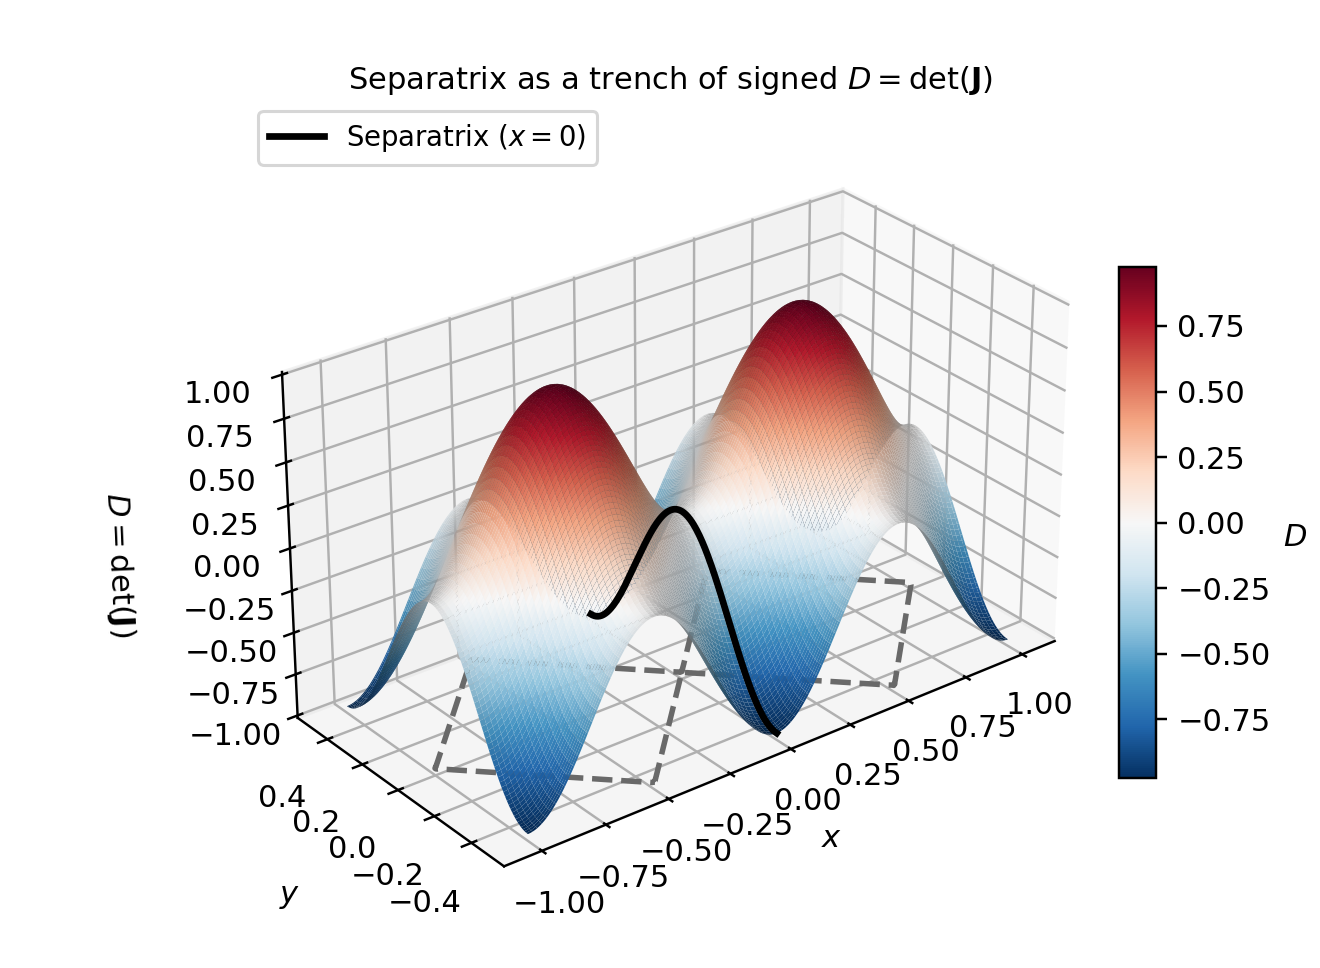
\includegraphics[width=0.36\textwidth]{figures/detJ_trench_cross_section.png}
    \caption{Signed $D$ as an elevation surface over the double gyre.
    The gyre cores rise as ridges ($D > 0$); the separatrix at $x = 0$
    (bold) is a valley of $D$, deepest at the saddles and rising to
    $D = 0$ at the origin.}
    \label{fig:trench_cross}
\end{figure}

\subsection{Problem Statement}
\label{sec:problem_statement}

Consider $N$ robots at positions $\mathbf{p}_i$, each measuring the
local flow $(u_i, v_i) = \mathbf{v}(\mathbf{p}_i)$ at the common
sampling instant, with no map, forecast, or prior field model and no
trajectory integration. The field is a number computed or replayed at
that instant, not a current the platform sits in: robot motion is
commanded by the control law, not advected by the sampled flow. Using
only the current synchronous samples at
each control cycle, the team must generate a centroid velocity command
$\dot{\mathbf{p}}_c$ that solves one of two problems, one per term of
(\ref{eq:splitting}):

\emph{Problem 1 (separatrix network traversal).} Drive the cluster
centroid onto the trench of $D$ and travel it, in the direction of the
ambient flow, through the saddle points where trench segments cross;
terminal capture at a single saddle is the special case in which the
selector's stationary-point test is tightened to stop the team there.

\emph{Problem 2 (objective network traversal).} Drive the centroid onto
the trench of $s_1$ and travel it, through the eigenvector swap where the
attracting and repelling segments meet, to a terminal attracting core
where the trench bottoms out, using only objective quantities throughout.

Both require, at minimum, pointwise estimates of the surrogate, its
gradient, and its curvature or eigenframe at the centroid. The next
section shows how a six-robot formation produces all of them from one
fit.

\section{Distributed Second-Order Estimation}
\label{sec:estimation}

\subsection{Quadratic Fit from Six Simultaneous Measurements}

Let $\mathbf{p}'_i = \mathbf{p}_i - \mathbf{p}_c$ denote robot positions
relative to the centroid and define the quadratic basis vector
\begin{equation}
    \boldsymbol{\phi}(\mathbf{p}') =
    \bigl[\,1, \; x', \; y', \; \tfrac{1}{2}{x'}^2, \;
    x' y', \; \tfrac{1}{2}{y'}^2\,\bigr]^\top,
    \label{eq:basis}
\end{equation}
whose one-half factors let the recovered coefficients estimate the Taylor
derivatives in (\ref{eq:quad_model_u})--(\ref{eq:quad_model_v}) directly,
with no rescaling. Stacking the six robots' basis vectors row-wise gives
the $6 \times 6$ formation matrix $\boldsymbol{\Phi}$, and the coefficient
estimates $\hat{\boldsymbol{\theta}}_u = [\hat{u}_0, \hat{u}_x,
\hat{u}_y, \hat{u}_{xx}, \hat{u}_{xy}, \hat{u}_{yy}]^\top$ and
$\hat{\boldsymbol{\theta}}_v$ solve
\begin{equation}
    \boldsymbol{\Phi}\,\hat{\boldsymbol{\theta}}_u = \mathbf{m}_u, \qquad
    \boldsymbol{\Phi}\,\hat{\boldsymbol{\theta}}_v = \mathbf{m}_v,
    \label{eq:solve}
\end{equation}
where $\mathbf{m}_u = [u_1, \ldots, u_6]^\top$ and
$\mathbf{m}_v = [v_1, \ldots, v_6]^\top$ collect the measurements, $u_i$
and $v_i$ being the field components sampled by robot $i$. One matrix
factorization serves both components. If the field is exactly quadratic
over the formation footprint, the $\mathcal{O}(\|\mathbf{p}'\|^3)$
remainder vanishes identically, and noise-free measurements give
$\hat{\boldsymbol{\theta}}_u = \boldsymbol{\theta}_u$ and
$\hat{\boldsymbol{\theta}}_v = \boldsymbol{\theta}_v$ for any nonsingular
$\boldsymbol{\Phi}$. On a general smooth field the remainder does not
vanish, and Section~\ref{sec:sensitivity} quantifies the bias it leaves
in the fit. The estimation is cooperative rather than distributed in the
consensus sense: it pools six position and velocity-field pairs, 24
scalars per cycle, at one common solver, not an iterative exchange among
peers.

\textit{Minimality:} each robot contributes one equation per component to
(\ref{eq:solve}), and each system has six unknowns, so a synchronous
sample from fewer than six robots leaves the unconstrained quadratic
model unidentifiable. The solution set is a positive-dimensional affine
subspace, and any method returning a single answer from five robots is
supplying a structural prior rather than reading one from the data. Such
a prior is available: imposing exact incompressibility ties $u_x + v_y =
0$ together with its two first derivatives, removing three coefficients,
and five robots then supply ten equations for nine unknowns. The
estimator fits the unconstrained model deliberately. Measured surface
currents are weakly divergent, the fitted divergence is a live diagnostic
rather than an assumption, and the sixth robot buys exactness over every
planar quadratic field rather than over a constrained subclass.

Six robots suffice exactly when $\boldsymbol{\Phi}$ is nonsingular, and
the singular formations admit a clean geometric description.

\begin{proposition}[Conic criterion]
\label{prop:conic}
$\boldsymbol{\Phi}$ is singular if and only if the six sampling points
lie on a common conic, including degenerate conics such as line pairs.
\end{proposition}

\begin{proof}
$\boldsymbol{\Phi}$ is singular exactly when
$\boldsymbol{\Phi}\mathbf{c} = \mathbf{0}$ for some nonzero
$\mathbf{c} \in \mathbb{R}^6$. Row $i$ of $\boldsymbol{\Phi}$ is
$\boldsymbol{\phi}(\mathbf{p}'_i)^\top$, so this holds if and only if
$\boldsymbol{\phi}(\mathbf{p}'_i)^\top \mathbf{c} = 0$ for every $i$,
that is, if and only if all six points lie on the zero set of the nonzero
quadratic polynomial $\boldsymbol{\phi}(\cdot)^\top \mathbf{c}$.
\end{proof}

The criterion carries a practical warning: any six robots on one circle,
a regular hexagon for example, are singular regardless of size or
orientation. Moving one robot to the center removes the degeneracy
entirely, because a conic vanishing at five points of a circle must be a
multiple of that circle, and a circle does not pass through its own
center. The resulting pentagon-plus-center shape, five robots on a ring
of radius $\rho$ at $72^\circ$ spacing and one at the center, is the
configuration \cite{15} derived for scalar Hessian estimation, whose
fixed symmetric weights are exact only for the ideal ring geometry and
bias the recovered Hessian under formation deformation. Solving
(\ref{eq:solve}) at the measured positions instead costs one
$6 \times 6$ factorization per cycle, negligible at 10~Hz, reused for
both components, and stays exact under any deformation short of the
conic degeneracy, with formation error entering only through the
conditioning $\kappa(\boldsymbol{\Phi})$, monitored online.

\subsection{Closed-Form Recovery of $D$, $\nabla D$, and $\mathbf{H}_D$}

The estimated Jacobian at the centroid is assembled from the linear
coefficients,
\begin{equation}
    \hat{\mathbf{J}}_0 =
    \begin{bmatrix}
        \hat{u}_x & \hat{u}_y \\ \hat{v}_x & \hat{v}_y
    \end{bmatrix},
    \qquad
    \hat{D}_0 = \hat{u}_x \hat{v}_y - \hat{u}_y \hat{v}_x.
    \label{eq:J_hat}
\end{equation}
Away from the centroid the fitted model makes every Jacobian entry affine
in $\mathbf{p}'$,
\begin{equation}
    \hat{\mathbf{J}}(\mathbf{p}) = \hat{\mathbf{J}}_0 +
    \begin{bmatrix}
        \hat{u}_{xx} x' + \hat{u}_{xy} y' &
        \hat{u}_{xy} x' + \hat{u}_{yy} y' \\
        \hat{v}_{xx} x' + \hat{v}_{xy} y' &
        \hat{v}_{xy} x' + \hat{v}_{yy} y'
    \end{bmatrix},
    \label{eq:jac_affine}
\end{equation}
so $\hat{D}(\mathbf{p}) = \det(\hat{\mathbf{J}}(\mathbf{p}))$ is an exactly
quadratic polynomial in $\mathbf{p}'$ over the footprint. Differentiating
it and evaluating at $\mathbf{p}' = \mathbf{0}$ gives the gradient and
Hessian at the centroid as polynomials in the fitted coefficients:
\begin{equation}
    \hat{\mathbf{g}}_0 =
    \begin{bmatrix}
        \hat{u}_{xx} \hat{v}_y + \hat{u}_x \hat{v}_{xy}
            - \hat{u}_{xy} \hat{v}_x - \hat{u}_y \hat{v}_{xx} \\
        \hat{u}_{xy} \hat{v}_y + \hat{u}_x \hat{v}_{yy}
            - \hat{u}_{yy} \hat{v}_x - \hat{u}_y \hat{v}_{xy}
    \end{bmatrix},
    \label{eq:grad_det}
\end{equation}
\begin{equation}
    \hat{\mathbf{H}}_{D,0} =
    \begin{bmatrix}
        2(\hat{u}_{xx} \hat{v}_{xy} - \hat{u}_{xy} \hat{v}_{xx}) &
        \hat{u}_{xx} \hat{v}_{yy} - \hat{u}_{yy} \hat{v}_{xx} \\
        \hat{u}_{xx} \hat{v}_{yy} - \hat{u}_{yy} \hat{v}_{xx} &
        2(\hat{u}_{xy} \hat{v}_{yy} - \hat{u}_{yy} \hat{v}_{xy})
    \end{bmatrix}.
    \label{eq:hess_det}
\end{equation}
Because $\hat{D}$ is quadratic, $\hat{\mathbf{H}}_{D,0}$ is independent of
position, the model reports the same curvature everywhere in the
footprint, and unlike the gradient it does not sharpen as the cluster
contracts onto the target.

The two quantities also differ in what the truncation costs them. Every
term of $\nabla D(\mathbf{p}_c)$ pairs a second derivative of the field
with a first derivative, so the quadratic model retains all of the field
data the true gradient depends on. The Hessian does not have that
property. Its $(1,1)$ entry expands as
\begin{equation}
    D_{xx} = 2(u_{xx} v_{xy} - u_{xy} v_{xx})
        + u_{xxx} v_y + u_x v_{xxy}
        - u_{xxy} v_x - u_y v_{xxx},
    \label{eq:Dxx_true}
\end{equation}
and (\ref{eq:hess_det}) keeps only the first pair. The four third-order
terms are set to zero by construction, not made small by a good fit;
Section~\ref{sec:sensitivity} quantifies the resulting bias. With the
estimated flow at the centroid, $\hat{\mathbf{v}}_0 = (\hat{u}_0,
\hat{v}_0)$, (\ref{eq:J_hat})--(\ref{eq:hess_det}) supply every quantity
the $D$ tracker consumes.

\subsection{Closed-Form Recovery of $s_1$ and the Strain Eigenframe}
\label{sec:s1_estimation}

The same fit supplies the objective quantities of
Section~\ref{sec:strain_field}. Writing $\mu = (u_x + v_y)/2$ (zero for
incompressible flow), $a = (u_x - v_y)/2$, and $b = (u_y + v_x)/2$ for
the mean, deviatoric normal, and shear strain, the strain eigenvalues
are $s_{1,2} = \mu \mp r$ with $r = \sqrt{a^2 + b^2}$, and the
eigenframe $(\mathbf{e}_1, \mathbf{e}_2)$ is that of the symmetric
matrix $\hat{\mathbf{S}}$ assembled from the linear coefficients. Under
the quadratic model, $\mu$, $a$, and $b$ are affine functions of
position, so the gradient of $\hat{s}_1$ is exact for the fitted field:
\begin{equation}
    \nabla \hat{s}_1 = \nabla\mu
    - \frac{a\,\nabla a + b\,\nabla b}{r},
    \label{eq:grad_s1}
\end{equation}
with $\nabla\mu$, $\nabla a$, $\nabla b$ read directly off the
second-order coefficients (for example $\nabla a = \tfrac{1}{2}(u_{xx} -
v_{xy},\; u_{xy} - v_{yy})^\top$). Two properties distinguish this
pipeline from the $D$ pipeline, one favorable and one prohibitive.

The favorable one: the tangent the $s_1$ tracker rides,
$\mathbf{e}_2$, comes from the \emph{first-order} fitted coefficients
(Lemma~\ref{lem:gains}), one full derivative order better in noise gain
than the $\hat{\mathbf{H}}_D$ eigenvectors the $D$ tracker uses for the
same purpose. Section~\ref{sec:results_oecs} quantifies the
difference by direct measurement.

\begin{remark}[No usable Hessian of $s_1$ exists under a quadratic fit]
\label{rem:s1hess}
The prohibitive one: a Newton step on $(\nabla \hat{s}_1,
\hat{\mathbf{H}}_{s_1})$ is impossible in principle, not merely
inaccurate. Under the quadratic model the map $\mathbf{p} \mapsto (a,
b)$ is affine, so $\hat{s}_1 = \mu - \|(a, b)\|$ is concave and its
Hessian is negative semidefinite \emph{for every field and every
formation}; the positive transverse curvature of an $s_1$ trench lives
in third derivatives of the velocity field, outside the span of any
quadratic fit. (On the double gyre, where $b \equiv 0$, the fitted
$\hat{\mathbf{H}}_{s_1}$ is numerically zero.) The gradient
(\ref{eq:grad_s1}) is unaffected: its transverse component recovers the
trench-restoring signal with the correct sign and order (fitted slope
$4.0$ against analytic curvature $6.9$).
\end{remark}

\subsection{Estimator Accuracy}
\label{sec:sensitivity}

Two independent noise channels perturb the samples available to the
estimator. Measurement noise is additive Gaussian on the $(u, v)$
components read by each robot:
\begin{equation}
    u_i^m = u(\mathbf{p}_i) + \eta_i^u, \quad
    v_i^m = v(\mathbf{p}_i) + \eta_i^v,
    \quad \eta \sim \mathcal{N}(0, \sigma_{uv}^2),
    \label{eq:meas_noise}
\end{equation}
with samples independent across robots, components, and time steps; this
is the sensor model of \cite{9}. Position noise perturbs the location at
which each robot samples the field,
\begin{equation}
    (u_i^m, v_i^m) = \mathbf{v}(\mathbf{p}_i + \boldsymbol{\xi}_i), \quad
    \boldsymbol{\xi}_i \sim \mathcal{N}(\mathbf{0}, \sigma_p^2 \mathbf{I}),
    \label{eq:pos_noise}
\end{equation}
while the quadratic fit (\ref{eq:solve}) uses the nominal positions
$\mathbf{p}_i$: the robot reads the field at a slightly wrong place,
inducing, to first order, an effective measurement error
$\mathbf{J}(\mathbf{p}_i)\,\boldsymbol{\xi}_i$ that couples the two
channels through the local Jacobian magnitude.

Measurement noise enters the coefficients directly: since
$\hat{\boldsymbol{\theta}}_u - \boldsymbol{\theta}_u =
\boldsymbol{\Phi}^{-1}\boldsymbol{\eta}$, each coefficient's standard
deviation is $\sigma_{uv}$ times the norm of the corresponding row of
$\boldsymbol{\Phi}^{-1}$, and for the pentagon-plus-center these norms
have closed form.

\begin{lemma}[Exact noise gains of the pentagon-plus-center formation]
\label{lem:gains}
For five robots on a ring of radius $\rho$ and one at the centroid, the
coefficient standard deviations are
\begin{equation}
    \sigma_{u_0} = \sigma_{uv}, \quad
    \sigma_{u_x} = \sigma_{u_y} = \frac{2}{\sqrt{10}}\frac{\sigma_{uv}}{\rho},
    \label{eq:gain_grad}
\end{equation}
\begin{equation}
    \sigma_{u_{xx}} = \sigma_{u_{yy}} = \frac{8}{\sqrt{10}}
    \frac{\sigma_{uv}}{\rho^2},
    \qquad
    \sigma_{u_{xy}} = \frac{4}{\sqrt{10}}\frac{\sigma_{uv}}{\rho^2},
    \label{eq:gain_hess}
\end{equation}
independent of the formation heading, and identically for
$\boldsymbol{\theta}_v$.
\end{lemma}

The proof, by direct inversion of $\boldsymbol{\Phi}$ using the fifth
roots of unity, is in Appendix~\ref{app:proofs}. Two consequences
follow. First, the gains are isotropic: the error covariance of the
estimated gradient is $\tfrac{4}{10}\sigma_{uv}^2\,\rho^{-2}\mathbf{I}$
for every heading, so estimator quality does not degrade as the cluster
turns. Second, each derivative order costs one power of the formation
radius, so larger formations average noise better. Truncation works the
other way: on a field with third derivatives bounded by $M_3$, the
Taylor remainder biases the fitted second-order coefficients by $O(M_3
\rho)$, matching the bound proved for the symmetric estimator in
\cite{15}, so smaller formations track curvature better. Balancing the two for the
second-order coefficients gives an optimal radius $\rho^* \propto
(\sigma_{uv}/M_3)^{1/3}$, a shallow cube-root bowl (Fig.~\ref{fig:est_accuracy}(b))
whose flat optimum is not computable in the field, since $M_3$ is a
property of an unknown flow and the exactly-determined six-robot fit
leaves no residual to estimate it from. The radius is fixed at $\rho =
0.075$ throughout this paper.

Propagating coefficient errors to the navigation quantities separates
cleanly by derivative order. The determinant obeys $|\hat{D} - D| \leq
\|\mathbf{J}\|_F \|\mathbf{E}\|_F + \tfrac{1}{2}\|\mathbf{E}\|_F^2$,
with $\mathbf{E} = \hat{\mathbf{J}} - \mathbf{J}$ the Jacobian error,
and the gradient formula (\ref{eq:grad_det}) inherits coefficient
errors linearly. The Hessian is different in kind: differentiating $D$
twice produces third derivatives of the field weighted by the field
itself, which a quadratic model cannot represent, so
(\ref{eq:hess_det}) is the Hessian of the fitted surface, not of $D$,
and carries a model bias that no formation size or averaging reduces.
For the double gyre at the nominal scale this bias is on the order of
$\|\mathbf{H}_D\|_F$ itself.

\begin{remark}[Hessian bias]
\label{rem:eigvec}
The controller of Section~\ref{sec:controllers} consumes
$\hat{\mathbf{H}}_D$ only through its eigenvectors and the signs and
rough magnitudes of its eigenvalues, and these degrade far less than
the Frobenius error suggests. Across the separatrix $D$ is even in the
transverse coordinate, so both the retained and the omitted terms are
diagonal in the trench frame: the estimated eigen-directions are exact
there to numerical precision and within a few degrees at generic
points, while the bias loads onto the eigenvalues, rescaling a Newton
snap that the saturation (\ref{eq:sat}) bounds and the closed loop
absorbs. This is why a formation too small to sense curvature
accurately can still track the structure that curvature defines. The
exception is the neighborhood of the wells, where the biased
eigenvalues nearly vanish and their signs become unreliable
(Section~\ref{sec:results}).
\end{remark}

\begin{figure}[!t]
    \centering
    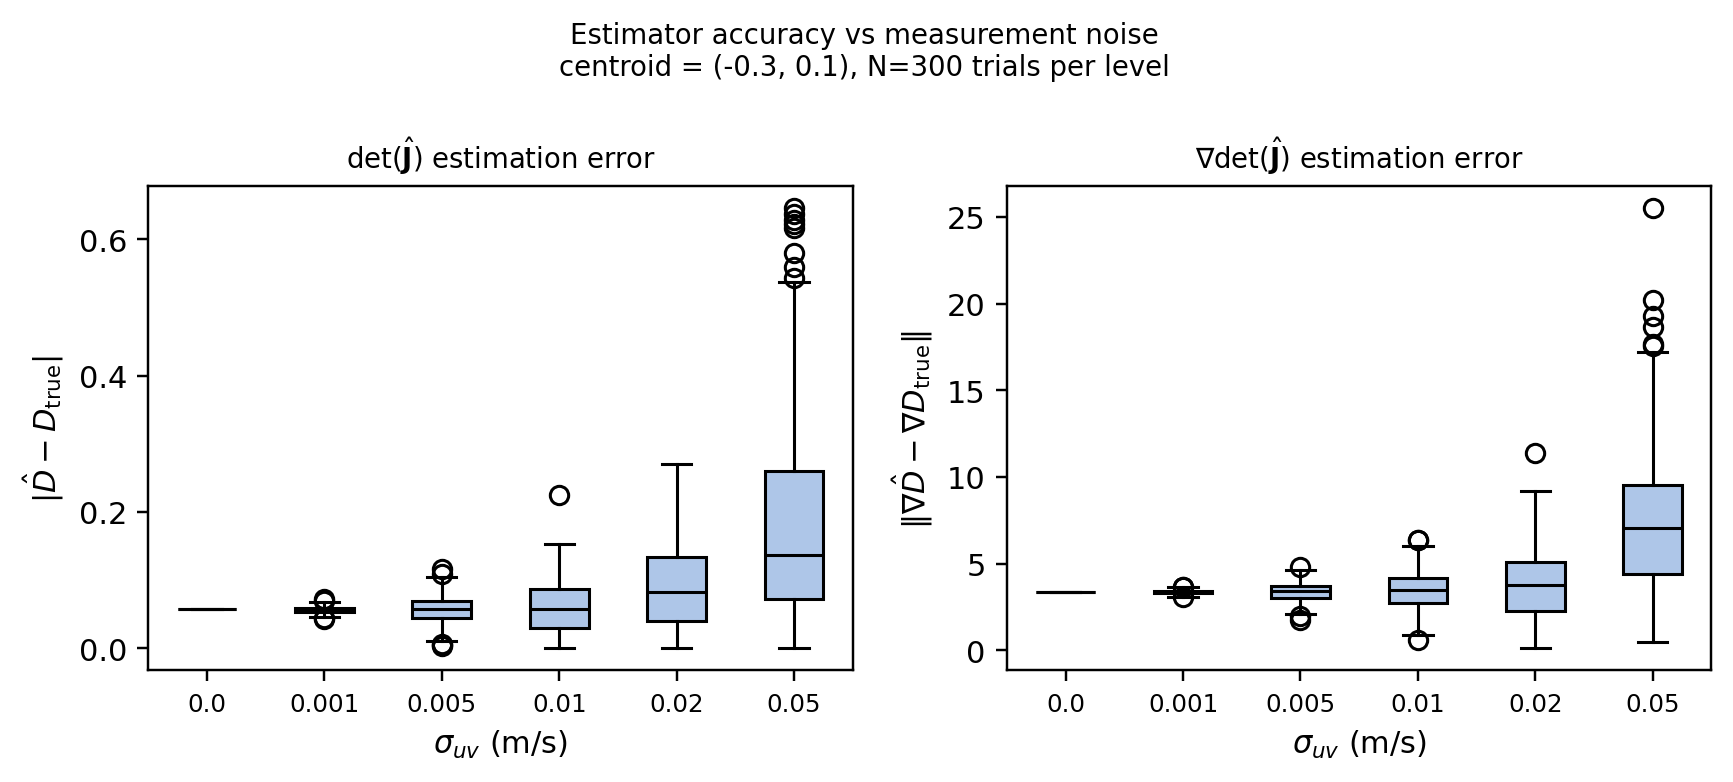
\includegraphics[width=0.34\textwidth]{figures/estimator_accuracy_vs_noise.png}
    \caption{Relative estimation error of $\hat{D}$, $\nabla\hat{D}$, and
    $\hat{\mathbf{H}}_D$ on the steady double gyre (median over $2 \times
    10^5$ noise draws per point; the dashed line marks error equal to
    signal). (a) Versus measurement noise at $\rho = 0.075$; the
    dash-dotted line marks the noise level where closed-loop traverse
    success crosses 50\% (Table~\ref{tab:mc_success}). (b) Versus
    formation radius at $\sigma_{uv} = 0.01$; dotted curves are the
    noise-free truncation floors.}
    \label{fig:est_accuracy}
\end{figure}

These predictions were checked open loop, holding the formation static
at a strain-region point of the double gyre over $2 \times 10^5$ noise
draws per condition. Every fitted coefficient's standard deviation
matched Lemma~\ref{lem:gains} within 0.3\%, and the position-noise
reading error matched its first-order prediction within 1.1\%,
confirming the two channels combine into a single effective measurement
noise. Reading the dashed-line crossings of Fig.~\ref{fig:est_accuracy}(a),
$\hat{D}$ stays informative to $\sigma_{uv} \approx 0.06$~m/s and
$\nabla\hat{D}$ to $\approx 0.01$~m/s, while $\hat{\mathbf{H}}_D$ sits at
the line even for the quietest sensors, held there by the structural
bias; its eigen-directions nevertheless remain accurate to $0.35^\circ$
on and near the separatrix and $3.8^\circ$ at the generic test point
(Remark~\ref{rem:eigvec}).

The gradient threshold marks where closed-loop degradation should
begin: at $\sigma_{uv} \approx 0.01$ a single $\nabla\hat{D}$ estimate
is as wrong as it is right. The closed loop does not extend this limit;
the Monte Carlo sweeps of Section~\ref{sec:results} place the tracker's
50\% success level exactly there.

\section{Adaptive Navigation Controllers}
\label{sec:controllers}

This section derives the two controllers. They share the estimation
step, the saturation idiom, and the three-layer architecture below;
everywhere they differ traces to which term of (\ref{eq:splitting}) the
tracker trusts, both terms for the $D$ tracker's network reach, the
strain term alone for the $s_1$ tracker's frame invariance.
Section~\ref{sec:objectivity_tradeoff} weighs the tradeoff.

\subsection{Multilayer Control Architecture}
\label{sec:arch}

The trackers run inside the layered control architecture of prior
cluster space control studies \cite{14,28,27,30}, shown in
Fig.~\ref{fig:control_architecture}. The adaptive navigation layer is
the only one that reads the field: each cycle it takes the six
synchronous position and velocity-field measurements (a separate
channel from robot actuation, per the modelling assumption of
Section~\ref{sec:problem_statement}), recovers the quantities of
Section~\ref{sec:estimation}, applies whichever tracker's control law
is active (Section~\ref{sec:sep_controller} or
Section~\ref{sec:oecs_controller}), and passes the desired centroid
velocity down. The cluster space layer holds the formation rigid
around that centroid command using a cluster-of-clusters
parameterization, robots grouped into three pairs (length $L$, angle
$\theta$ each) whose midpoints form a Side-Angle-Side triangle
\cite{31}, twelve shape variables in place of the twelve Cartesian
coordinates, regulated to the pentagon-plus-center nominal
(Corollary~\ref{cor:pentagon}) except the centroid and heading, which
the top layer's command alone determines. This is the layer where the
two trackers of this paper actually differ from each other: everything
beneath it is a fixed, tracker-agnostic mechanism, so replacing the $D$
tracker with the $s_1$ tracker changes nothing about the two layers
beneath it.

\begin{figure}[!t]
    \centering
    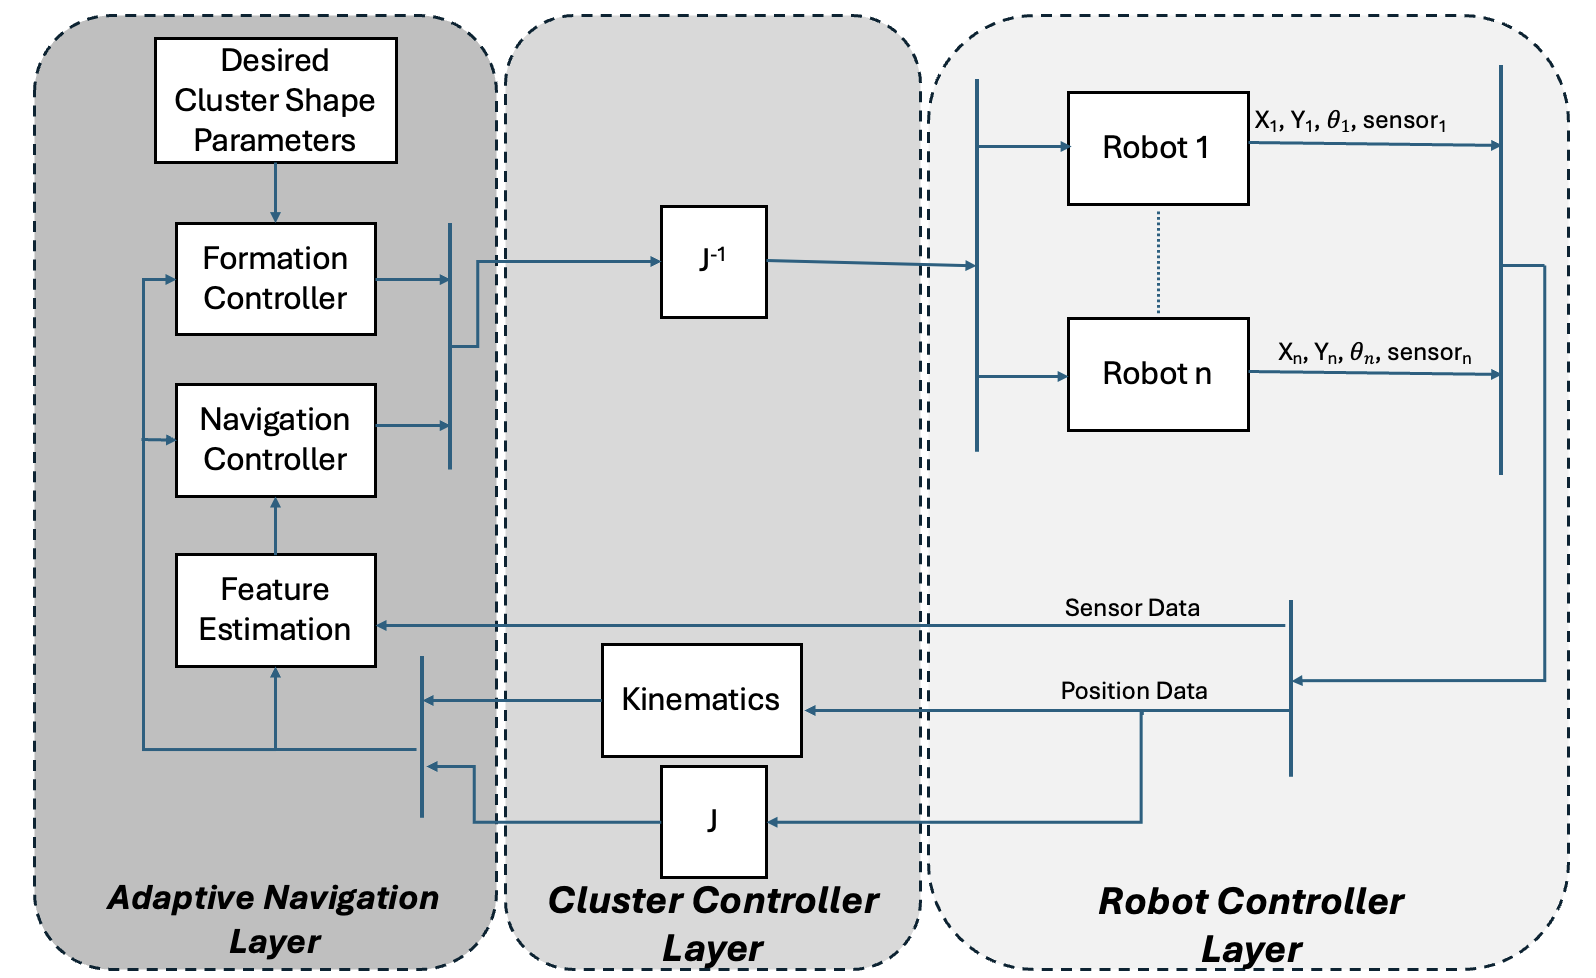
\includegraphics[width=0.40\textwidth]{figures/control_architecture.png}
    \caption{Hierarchical control architecture: robot, cluster space,
    and adaptive navigation layers.}
    \label{fig:control_architecture}
\end{figure}

\subsection{The Modified Newton Step}
\label{sec:mod_newton}

Under the quadratic model, $\hat{D}(\mathbf{p})$ is an exact quadratic
surface with gradient $\hat{\mathbf{g}}$ and constant Hessian
$\hat{\mathbf{H}}_D$, so the natural navigation move is the Newton step
$-\hat{\mathbf{H}}_D^{-1}\hat{\mathbf{g}}$, which in the eigenbasis
$\hat{\mathbf{H}}_D \mathbf{w}_k = \lambda_k \mathbf{w}_k$ ($\lambda_1
\leq \lambda_2$ throughout) has per-direction components
$-(\mathbf{w}_k^\top \hat{\mathbf{g}})/\lambda_k$. As a velocity
command the raw step fails twice: its magnitude explodes where
$\hat{\mathbf{H}}_D$ is near singular, and it converges to whatever
stationary point the local model exhibits, climbing a trench wherever
the along-trench curvature is negative. Componentwise saturation
through
\begin{equation}
    \mathrm{sat}(c) = v_{\max} \tanh\!\left(\frac{c}{v_{\max}}\right)
    \label{eq:sat}
\end{equation}
repairs the first defect, giving the \emph{attract step}
\begin{equation}
    \dot{\mathbf{p}}_c = \sum_{k=1}^{2}
    \mathrm{sat}\!\left(-\frac{\mathbf{w}_k^\top
    \hat{\mathbf{g}}}{\lambda_k}\right)\mathbf{w}_k,
    \label{eq:attract_step}
\end{equation}
a bounded constant-speed reach far from the structure that recovers the
exact Newton component, with its superlinear local convergence, once
the argument is small; the one parameter $v_{\max}$ sets both the
cruise speed and the terminal boundary layer. Replacing each eigenvalue
by its magnitude, the saddle-free Newton modification of \cite{35},
repairs the second, giving the \emph{slide step}
\begin{equation}
    \dot{\mathbf{p}}_c = \sum_{k=1}^{2}
    \mathrm{sat}\!\left(-\frac{\mathbf{w}_k^\top
    \hat{\mathbf{g}}}{|\lambda_k|}\right)\mathbf{w}_k,
    \label{eq:slide_step}
\end{equation}
which agrees with (\ref{eq:attract_step}) in directions of positive
curvature, snapping the centroid onto the trench floor, and reverses
the Newton component into a curvature-normalized descent along the
trench, away from crests, in the direction of negative curvature. Every
term of both laws is quadratic in $\mathbf{w}_k$, so the sign ambiguity
of eigenvectors leaves the commands unchanged.

\subsection{The $D$ Tracker}
\label{sec:sep_controller}

The $D$ tracker composes the two step bodies with a third,
flow-assisted mode, needed because the slide step descends $D$ and
therefore stalls at the crest, where the along-trench gradient
vanishes, while the separatrix continues through it. On the separatrix
the ambient flow is tangent to the structure and nonzero away from the
saddles, so the flow can carry the team across. The cluster is declared
on the separatrix (FLOW band) when either
\begin{equation}
    |\hat{D}| < \varepsilon_{\text{raw}}
    \quad\text{or}\quad
    \frac{|\hat{D}|}{\|\hat{\mathbf{H}}_D\|_F} < \varepsilon_{\text{dim}},
    \label{eq:flow_band}
\end{equation}
where $\varepsilon_{\text{raw}}$ is a raw threshold and
$\varepsilon_{\text{dim}}$ a curvature-normalized threshold (units of
length squared) that makes the band scale with the local landscape. In
the FLOW band the command follows the measured flow along the trench
tangent $\mathbf{w}_1$ and retains the Newton snap across it: the
\emph{flow step} is
\begin{equation}
    \dot{\mathbf{p}}_c =
    \mathrm{sat}\!\left(\mathbf{f}^\top \mathbf{w}_1\right)\mathbf{w}_1
    + \mathrm{sat}\!\left(-\frac{\hat{\mathbf{g}}^\top
    \mathbf{w}_2}{\lambda_2}\right)\mathbf{w}_2.
    \label{eq:flow_step}
\end{equation}
Off the band, with $\mathbf{w}_1$ oriented so that
$\hat{\mathbf{g}}^\top \mathbf{w}_1 \leq 0$ (descent along the
trench), the complete control law, with cases evaluated in order once
per cycle, is
\begin{equation}
    \dot{\mathbf{p}}_c =
    \begin{cases}
        \text{flow (\ref{eq:flow_step})}, &
            \text{(\ref{eq:flow_band}) holds (FLOW)}, \\[1pt]
        \text{attract (\ref{eq:attract_step})}, &
            \lambda_1\lambda_2 \geq 0 \ \text{or}\
            \mathbf{f}^\top\mathbf{w}_1 \leq 0 \ \text{(ATTRACT)}, \\[1pt]
        \text{slide (\ref{eq:slide_step})}, &
            \text{otherwise (SLIDE)}.
    \end{cases}
    \label{eq:d_selector}
\end{equation}
The ATTRACT case carries the terminal behaviors inline:
$\lambda_1\lambda_2 \geq 0$ is the stationary-point (capture) test,
satisfied near a well of $D$, where the attract step becomes the
terminal capture law of Theorem~\ref{thm:attract}, the sub-case
Sections~\ref{sec:results} and~\ref{sec:discussion} call the
\emph{attract fallback}; and
$\mathbf{f}^\top\mathbf{w}_1 \leq 0$ catches upstream starts, for
which the attract step climbs to the crest, whose FLOW band hands the
team to the flow. Both sub-cases and the flow-drift guard of the next
paragraph are refinements inside the three named modes, not additional
entries in the switching law itself. In all three modes the tangential motion is never
directed against the ambient flow.

One guard is not shown in (\ref{eq:d_selector}): inside the band, if $\hat{\mathbf{H}}_D$ has no
saddle structure, the command falls back to the saturated flow alone;
with exact estimates this cannot occur on the trench away from the band
boundary, and Section~\ref{sec:results} counts it as the flow-drift
refinement. Note that the $\mathbf{w}_2$ component is one and the same
in all three laws: on a trench $\lambda_2 > 0$, so the signed and
magnitude denominators agree and every mode applies the identical
transverse Newton snap. The modes differ only in their motion along the
structure, which is what makes the switched system tractable in
Section~\ref{sec:stability}.

\subsection{The $s_1$ Tracker}
\label{sec:oecs_controller}

The case for a second controller is not that $D$ is wrong, but that it
is not a property of the material: by (\ref{eq:splitting}), $D$ mixes
the strain term with the spin term $\omega^2/4$, and
(\ref{eq:D_not_objective}) shows a platform rotating at $\Omega$
relative to the one the field was recorded in sees a different scalar
field, with different trenches, saddles, and crossings, from the same
physical water. The strain term alone does not carry this: $s_1$ is an
eigenvalue of $\mathbf{S} = (\mathbf{J} + \mathbf{J}^\top)/2$, which
transforms as $\mathbf{S}' = \mathbf{Q}\mathbf{S}\mathbf{Q}^\top$ under
any rotation of the observer, so its eigenvalues are exactly invariant
and its eigenframe co-rotates, on both the attracting segment (tangent
to $\mathbf{e}_2$) and the repelling one (tangent to $\mathbf{e}_1$,
Section~\ref{sec:dg_example}) alike: the same guarantee Serra and
Haller's attracting OECSs and the TRAP-core search-and-rescue
literature build on \cite{17,36}. The second
controller developed here
asks whether that guarantee is reachable with the same cooperative,
map-free, single-sample estimator the $D$ tracker uses, riding the same
separatrix network rather than a bounded segment of it
(Section~\ref{sec:results_oecs}). Section~\ref{sec:objectivity_tradeoff}
and Section~\ref{sec:limitations} report what that guarantee costs at
this paper's own test point.

The second controller traverses the trench of $s_1$
(Section~\ref{sec:strain_field}) using only the objective quantities the
fit delivers: $\hat{s}_1$, $\nabla\hat{s}_1$, the deviatoric strain
magnitude $r$, and the strain eigenframe $(\mathbf{e}_1, \mathbf{e}_2)$.
Remark~\ref{rem:s1hess} rules out a Newton snap, so both channels are
built from the gradient rather than the curvature. The trench is
transverse on both separatrix halves (Section~\ref{sec:dg_example}), and
which eigenvector is tangent to it swaps at the degeneracy lines, so
neither channel names an eigenvector directly; instead, away from a
stationary point of $s_1$ the gradient itself resolves the split, since
the transverse derivative vanishes on the trench by construction and
$\nabla\hat{s}_1$ points almost entirely along it:
\begin{equation}
    \hat{d}_1 = \bigl\lvert \nabla\hat{s}_1^\top \mathbf{e}_1
    \bigr\rvert, \qquad
    \hat{d}_2 = \bigl\lvert \nabla\hat{s}_1^\top \mathbf{e}_2
    \bigr\rvert,
    \label{eq:d1d2}
\end{equation}
\begin{equation}
    \hat{\mathbf{t}} = \mathrm{sign}\bigl(\mathbf{t}_{\text{ref}}^\top
    \mathbf{t}_{\text{raw}}\bigr)\,\mathbf{t}_{\text{raw}}, \qquad
    \mathbf{t}_{\text{raw}} = \begin{cases}
        \mathbf{e}_1, & \hat{d}_1 \geq \hat{d}_2, \\
        \mathbf{e}_2, & \hat{d}_1 < \hat{d}_2,
    \end{cases}
    \label{eq:tangent_select}
\end{equation}
with $\mathbf{t}_{\text{ref}}$ the previous step's tangent
$\mathbf{t}_{\text{prev}}$ once established, or the measured flow
$\mathbf{f}$ on the first tracking step. The larger of
(\ref{eq:d1d2}) is the tangent, matching the verified geometry: it
selects $\mathbf{e}_2$ on the attracting half and $\mathbf{e}_1$ on the
repelling half, swapping automatically through the origin, and it is
this same pair that resolves which trench branch to continue onto at a
crossing, since the crossing wall trench has its own, different larger
projection. Continuity with $\mathbf{t}_{\text{prev}}$ fixes only the
residual sign; the direction itself never depends on it, and TRACK never
consults the flow past its own first invocation
(Proposition~\ref{prop:equivariance}); CROSS does read the flow directly,
guarded by $r < r_{\text{band}}$ and reachable only on the very first
tracking step. The transverse channel descends
$\hat{s}_1$ along whichever component (\ref{eq:d1d2}) did not select,
\begin{equation}
    \dot{\mathbf{p}}_c^{\,\perp} =
    \mathrm{sat}\!\bigl(-g_\perp\,\nabla\hat{s}_1^\top
    \hat{\mathbf{n}}\bigr)\,\hat{\mathbf{n}}, \qquad
    \hat{\mathbf{n}} = \begin{cases}
        \mathbf{e}_2, & \hat{\mathbf{t}} = \pm\mathbf{e}_1, \\
        \mathbf{e}_1, & \hat{\mathbf{t}} = \pm\mathbf{e}_2,
    \end{cases}
    \label{eq:oecs_perp}
\end{equation}
a saturated gradient step with fixed gain $g_\perp$ in place of the
unavailable curvature normalization; on the trench the argument is a
restoring signal whose slope is the true transverse curvature, so
(\ref{eq:oecs_perp}) contracts at gradient rate rather than Newton
rate, the first cost of objectivity. The tangential channel rides at
constant cruise speed, $\dot{\mathbf{p}}_c^{\,\parallel} =
v_{\max}\tanh(1)\,\hat{\mathbf{t}}$. Both channels are built from the
same two projections (\ref{eq:d1d2}), so no third estimated quantity
enters the ride. A flow saddle is not merely a crossing of two
transverse trenches; it is a genuine two-dimensional local minimum of
$s_1$ (verified numerically: the true Hessian of $s_1$ has both
eigenvalues strictly positive there, $s_1'' \approx 9.7$ at the
double-gyre saddle, consistent with the well depth $s_1 = -\pi^2 A$),
so $\nabla\hat{s}_1$ vanishes in \emph{every} direction, not only
transversally, and this distinguishes it cleanly from an ordinary
trench point, where the gradient stays large along the trench even
though it vanishes across it. This matters because the ambient flow
also collapses at a saddle, a stagnation point of the flow itself, so a
tangent rule built from the flow would be starved of a reliable
direction exactly where the ride most needs one; testing the gradient
magnitude directly sidesteps the ambiguity entirely. The complete
control law, with cases evaluated in order once per cycle, is
\begin{equation}
    \dot{\mathbf{p}}_c =
    \begin{cases}
        -\mathrm{sat}(g_\perp\nabla\hat{s}_1), &
            \text{pre-band (ACQUIRE)}, \\[1pt]
        -\mathrm{sat}(g_\perp\nabla\hat{s}_1), &
            \hat{s}_1 < s_{\text{capture}}\ \text{(PARK)}, \\[1pt]
        -\mathrm{sat}(g_\perp\nabla\hat{s}_1), &
            \lVert\nabla\hat{s}_1\rVert < g_{\text{capture}}\
            \text{(CAPTURE)}, \\[1pt]
        v_{\max}\tanh(1)\,\hat{\mathbf{f}} + \dot{\mathbf{p}}_c^{\,\perp},
            & r < r_{\text{band}}\ \text{(CROSS)}, \\[1pt]
        \dot{\mathbf{p}}_c^{\,\perp} +
            \dot{\mathbf{p}}_c^{\,\parallel}, &
            \text{otherwise (TRACK)},
    \end{cases}
    \label{eq:oecs_selector}
\end{equation}
where the saturation in the ACQUIRE, PARK, and CAPTURE cases acts
componentwise on the gradient, $s_{\text{trim}} > 0$ is the
attraction-dominance threshold that marks the ride as having reached
genuine structure rather than a noise fluctuation, the flag banded
latches once $\hat{s}_1 < -s_{\text{trim}}$ first holds, and PARK is active only
when $s_{\text{capture}}$ is set (default: unset). CAPTURE needs no
field-specific value the way PARK does, but it is not unconditional: it
is guarded by $r > r_{\text{band}}$ so it is not confused with the
isotropic point, where the gradient can be small for a different
reason, and, once fired, it is latched until $\hat{s}_1$ rises back
above $-s_{\text{trim}}$, which bridges a noise-driven flicker of the
gradient test at the well without holding past a genuine departure from
it, a bounded latch distinct from the banded flag's own, unbounded one.
CROSS, reached only on the very first tracking step if $r <
r_{\text{band}}$ with no prior tangent to fall back on, rides the flow
directly and is essentially unreachable once tracking is underway,
since ACQUIRE's gradient descent lands on-trench well before $r$ drops
this low with no established tangent. TRACK's own tangent selection
also reads the flow, but only once: on its first invocation, if CROSS
was not reached, $\mathbf{t}_{\text{ref}}$ in (\ref{eq:tangent_select})
falls back to the measured flow to fix the initial sign, exactly as the
sign of the $D$ tracker's own ride tangent is seeded
(Section~\ref{sec:sep_controller}); every subsequent step resolves the
sign from $\mathbf{t}_{\text{prev}}$ alone. The cases carry the terminal
behavior inline: ACQUIRE descends $\hat{s}_1$ toward stronger attraction
before first structure contact; PARK settles early inside a core well if
a threshold is supplied; CAPTURE settles at any two-dimensional
stationary point of $\hat{s}_1$ the ride reaches, the default terminal
behavior with no field-specific threshold to set.

CAPTURE plays the role the capture test plays in the $D$ tracker, but
where $D_{\text{capture}}$ (Section~\ref{sec:park_vs_traverse}) is an
opt-in threshold the user sets to override the base selector's
continuation, CAPTURE fires by default and needs no field-specific
value: it holds any two-dimensional stationary point the objective
gradient finds. Every quantity the selector consumes transforms
equivariantly under a time-dependent rotation of the observer
(Proposition~\ref{prop:equivariance}), so in ACQUIRE, PARK, CAPTURE, and
both channels of TRACK the commanded velocity co-rotates and the
closed-loop trajectory is the same material path in any frame, with one
exception confined to a single instant: on TRACK's first invocation, if
no previous tangent has yet been established (CROSS was not reached),
the sign reference falls back to the measured flow, exactly as the $D$
tracker's own ride mode seeds its tangent; thereafter orientation is
carried forward by continuity alone, which is covariant, for the
remainder of the run. This is a stronger objectivity claim than a
design built on continuity alone would give, and no weaker than the $D$
tracker's own ride mode: continuity fixes only a sign, so a rule that
instead resolved (\ref{eq:tangent_select}) by best alignment with the
flow at every step, mirroring the $D$ tracker's own flow test in
(\ref{eq:d_selector}), would inherit the flow's dependence on the
observer frame at every step, not merely once, at the seed. What the controller
gives up is explicit and gradient-rate throughout, not merely at the
transverse channel: it traverses the full separatrix, through the
eigenvector swap and the network crossing alike, using no Newton step
and, in TRACK, no flow. Section~\ref{sec:results} shows both sides.

\subsection{Stability Properties}
\label{sec:stability}

The analysis is carried out at the navigation level: the cluster
centroid is modeled as a kinematic integrator
\begin{equation}
    \dot{\mathbf{p}}_c = k\,\boldsymbol{\delta}(\mathbf{p}_c),
    \label{eq:kinematic_model}
\end{equation}
where $\boldsymbol{\delta}$ is the right-hand side of the active
control law, (\ref{eq:d_selector}) or (\ref{eq:oecs_selector}), and
$k > 0$ is the navigation gain (time is rescaled so $k = 1$). The
results below are continuous-time; the simulator advances
(\ref{eq:kinematic_model}) by explicit Euler at $\Delta t = 0.1$~s with
$k = 3.0$ (double gyre) or $k = 1.8$ (ocean), so the per-step
contraction is only conditionally guaranteed by this analysis and was
instead verified numerically at both operating points: the noise-free
runs of Section~\ref{sec:results} converge without overshoot or
oscillation at the reported gains. This abstracts the
cluster and robot layers, whose tracking dynamics are an order of
magnitude faster ($\tau \approx 0.3$~s against transit times of tens of
seconds), a separation validated in hardware in \cite{14}. Estimates
are taken exact unless stated otherwise; $\mathbf{w}_1, \mathbf{w}_2$
denote unit eigenvectors of $\mathbf{H}_D$ with $\lambda_1 \leq
\lambda_2$, and $z_k = (\mathbf{w}_k^\top \mathbf{g})/\lambda_k$ are
the Newton components. All proofs are collected in
Appendix~\ref{app:proofs}.

The first result certifies the attract step globally, wherever
$\mathbf{H}_D$ is nonsingular.

\begin{theorem}[Attract-mode certificate]
\label{thm:attract}
Let $V_A = \tfrac{1}{2}\|\mathbf{g}(\mathbf{p}_c)\|^2$. Along
(\ref{eq:kinematic_model}) with the attract step
(\ref{eq:attract_step}),
\begin{equation}
    \dot{V}_A = -v_{\max} \sum_{k=1}^{2} \lambda_k^2\,
    z_k \tanh\!\left(\frac{z_k}{v_{\max}}\right) \;\leq\; 0,
    \label{eq:VA_dot}
\end{equation}
with equality exactly where $\mathbf{g} = \mathbf{0}$. Consequently
every bounded trajectory on which $\mathbf{H}_D$ remains nonsingular
converges to the critical set $\{\mathbf{g} = \mathbf{0}\}$ of $D$, and
isolated critical points with $\mathbf{H}_D$ nonsingular are locally
exponentially stable.
\end{theorem}

Far from the trench the attract step is the approach law, descending
$\|\nabla D\|^2$ toward the stationary set of $D$; near a well of $D$,
where $\mathbf{H}_D \succ 0$, it is the terminal capture law, and
convergence is exponential.

For the traversal result the trench is formalized as a valley line with
a flow along it.

\begin{assumption}[Trench and flow structure]
\label{ass:trench}
There is a segment $\Gamma$ with tangent $\hat{\mathbf{e}}_\parallel$,
normal $\hat{\mathbf{e}}_\perp$, arclength coordinates $(\ell, n)$, and
a tube $T_w = \{|n| \leq w\}$ on which: (i)
\begin{equation}
    D(\ell, n) = h(\ell) + \tfrac{1}{2}\lambda_\perp(\ell)\,n^2,
    \qquad 0 < \underline{\lambda} \leq \lambda_\perp(\ell),
    \label{eq:normal_form}
\end{equation}
with vanishing cross terms
($\hat{\mathbf{e}}_\perp^\top \mathbf{H}_D \hat{\mathbf{e}}_\parallel
= 0$ on $T_w$) and eigenvalue gap $\lambda_2 - \lambda_1 \geq \gamma >
0$ wherever the selector is outside its attract fallback; and (ii)
$\Gamma$ is an invariant curve of the flow, with $\|\mathbf{v}\| \geq
f_{\min} > 0$ outside balls of radius $r_0$ around the flow saddles,
and the stationary points of $h$ are wells at the flow saddles
and crests inside the FLOW band, with $|h'(\ell)| \geq m_h >
0$ wherever the band test fails on $\Gamma$.
\end{assumption}

The cross-term condition holds exactly for additively separable
fields, the double gyre among them; for $\ell$-dependent $\lambda_\perp$
the residual cross term $\lambda_\perp'(\ell)\,n$ enters the transverse
channel as a bounded disturbance covered by
Proposition~\ref{prop:iss}.

The double-gyre separatrix satisfies Assumption~\ref{ass:trench} with
$n = x$, $\ell = y$: the field (\ref{eq:det_analytic_main}) is additively
separable, so the cross terms vanish identically and the transverse
curvature is positive on any tube with $w < 1/4$; the appendix shows the
higher-order terms only strengthen the contraction.

Two appendix lemmas carry the proof: every selector mode applies the
identical transverse contraction
\begin{equation}
    \dot{n} = -v_{\max}\tanh\!\left(\frac{n}{v_{\max}}\right),
    \label{eq:n_dynamics}
\end{equation}
so the tube is forward invariant and mode switching cannot chatter it
(Lemma~\ref{lem:transverse}), and no mode moves against the ambient flow
along the trench, with tangential speed at least $m > 0$ outside the
$r_0$ balls (Lemma~\ref{lem:progress}).

\begin{theorem}[Separatrix network traversal]
\label{thm:separatrix}
Under Assumption~\ref{ass:trench}, with exact estimates, every
trajectory of the $D$ tracker starting in the tube $T_w$ (i) remains in
$T_w$ and converges exponentially to the trench, and (ii) traverses the
trench in the direction of the ambient flow, reaching the $r_0$
neighborhood of a flow saddle in finite time bounded by $L_\Gamma/m$,
with $L_\Gamma$ the trench length and $m$ the progress rate of
Lemma~\ref{lem:progress}. At the saddle, $D$ attains a local minimum
with $\mathbf{H}_D \succ 0$, the selector's stationary-point test
$\lambda_1\lambda_2 \geq 0$ is satisfied, and (iii)
Theorem~\ref{thm:attract} gives local exponential convergence to the
saddle: terminal capture.
\end{theorem}

\begin{remark}[Capture depends on the estimated Hessian]
\label{rem:capture_gap}
The trench is not a single arc: the saddle is a crossing of two
perpendicular trench segments (Section~\ref{sec:dg_example}), so a
selector that reaches the ball without certifying $\mathbf{H}_D \succ
0$ remains in its flow or slide modes and continues onto the crossing
segment, repeating (i)-(ii) with $\Gamma$ relabeled.
Remark~\ref{rem:eigvec} says exactly when this happens: near the wells
the biased eigenvalues nearly vanish and their signs become unreliable,
so the test does not fire on $\hat{\mathbf{H}}_D$ even without noise,
and the selector takes continuation rather than capture, as
Section~\ref{sec:results} confirms at every saddle reached. Tightening
the test recovers capture (Section~\ref{sec:discussion}); both
behaviors are the same theorem applied to different premises at the
crossing.
\end{remark}

Robustness to estimation error follows from the saturation structure:
every command channel passes its argument through a $\tanh$, which is
1-Lipschitz, so bounded estimate perturbations become bounded command
disturbances.

\begin{proposition}[Ultimate bound under bounded estimate error]
\label{prop:iss}
Suppose the estimate errors induce a bounded disturbance $d(t)$, $|d|
\leq \bar{d} < v_{\max}$, in the transverse channel, so that
(\ref{eq:n_dynamics}) becomes $\dot{n} = -v_{\max}\tanh(n/v_{\max}) +
d$. Then the trench remains practically stable with ultimate bound
\begin{equation}
    \limsup_{t\to\infty} |n(t)| \;\leq\;
    v_{\max}\operatorname{artanh}\!\left(\frac{\bar{d}}{v_{\max}}\right),
    \label{eq:iss_bound}
\end{equation}
which is $\approx \bar{d}$ for $\bar{d} \ll v_{\max}$.\footnote{Proof:
$\tfrac{d}{dt}\tfrac{1}{2}n^2 = n(-v_{\max}\tanh(n/v_{\max}) + d) < 0$
whenever $v_{\max}\tanh(|n|/v_{\max}) > \bar{d}$, that is outside the
stated interval, which is therefore attractive and invariant.}
\end{proposition}

The disturbance level $\bar{d}$ inherits the noise and truncation
scalings of Section~\ref{sec:sensitivity}, so the bound
(\ref{eq:iss_bound}) degrades linearly in the measurement noise level;
the Monte Carlo sweeps described in Section~\ref{sec:test_plan} and
reported in Section~\ref{sec:results} quantify these predictions
empirically.

For the $s_1$ tracker, two properties are stated at the same
navigation level.

\begin{proposition}[Frame equivariance of the closed loop]
\label{prop:equivariance}
Let $\mathbf{p}'= \mathbf{Q}(t)\mathbf{p}$ be a time-dependent rotation
of the observer frame, and let the tracker of
Section~\ref{sec:oecs_controller} run on the transformed field
$\mathbf{v}'(\mathbf{p}', t) = \mathbf{Q}\mathbf{v}(\mathbf{Q}^\top
\mathbf{p}', t) + \dot{\mathbf{Q}}\mathbf{Q}^\top\mathbf{p}'$ with
exact estimates. Then the selector branch chosen at each state is the
same in both frames, and in the PARK, CAPTURE, and both channels of
TRACK the commanded velocity transforms as
$\boldsymbol{\delta}' = \mathbf{Q}\boldsymbol{\delta}$, so the
closed-loop navigation trajectory (\ref{eq:kinematic_model}) satisfies
$\mathbf{p}'_c(t) = \mathbf{Q}(t)\mathbf{p}_c(t)$ up to the
frame-transport term: on the structure, the tracker follows the same
material path in every frame. This includes the tangent selection
(\ref{eq:tangent_select}), built from $\nabla\hat{s}_1$ and the
co-rotating eigenframe alone, so the selected eigenvector and its
continuity-inherited sign both co-rotate with $\mathbf{Q}$. The two
branches that are not covariant are confined and harmless: ACQUIRE
saturates in observer axes but descends the invariant $\hat{s}_1$ in
every frame, a frame-dependent transient the contraction
(\ref{eq:oecs_n_dynamics}) absorbs; CROSS reads the flow directly but is
reached only on the first tracking step under an already-degenerate
eigenframe, essentially never in practice
(Section~\ref{sec:oecs_controller}).
\end{proposition}

For local convergence, the transverse channel replaces the common
Newton snap of Lemma~\ref{lem:transverse} with the saturated gradient
step (\ref{eq:oecs_perp}). On a trench of $s_1$ satisfying the analogue
of Assumption~\ref{ass:trench}, $s_1(\ell, n) = h_1(\ell) +
\tfrac{1}{2}\kappa_\perp(\ell)\,n^2$ with $0 < \underline{\kappa} \leq
\kappa_\perp$, the transverse coordinate obeys
\begin{equation}
    \dot{n} = -v_{\max}\tanh\!\left(
    \frac{g_\perp \kappa_\perp(\ell)\,n}{v_{\max}}\right),
    \label{eq:oecs_n_dynamics}
\end{equation}
the same saturated scalar contraction as (\ref{eq:n_dynamics}) with the
unit Newton rate replaced by the field-dependent rate $g_\perp
\kappa_\perp$: exponential once $|n| \leq v_{\max}/(g_\perp
\underline{\kappa})$, with rate proportional to the local curvature
rather than normalized by it. Because $\hat{\mathbf{n}}$ is whichever
eigenvector (\ref{eq:tangent_select}) did not select as tangent, this
holds on both separatrix halves without change, the transverse identity
swapping along with the tangent's. The disturbance analysis of
Proposition~\ref{prop:iss} carries over verbatim with $\bar{d}$ now the
error in $g_\perp \nabla\hat{s}_1^\top\hat{\mathbf{n}}$.

Termination is by CAPTURE rather than by a boundary condition:
componentwise saturated descent of $\hat{s}_1$ carries its own
certificate independent of the transverse-channel argument above,
since under exact estimates $s_1$ itself is a Lyapunov function for the
full gradient,
\begin{equation}
    \dot{\hat{s}}_1 = -\sum_k (\partial_k \hat{s}_1)\,
    \mathrm{sat}(g_\perp\,\partial_k \hat{s}_1) \leq 0,
    \label{eq:s1_lyapunov}
\end{equation}
with equality only at a critical point of $\hat{s}_1$, the same descent
ACQUIRE and PARK apply; CAPTURE differs only in its trigger,
$\lVert\nabla\hat{s}_1\rVert < g_{\text{capture}}$, which fires at any
network minimum. Unlike the $D$ tracker's Hessian-based test, unreliable
at a saddle (Remark~\ref{rem:capture_gap}), (\ref{eq:s1_lyapunov}) needs
no curvature estimate: the saddle is recoverable as a two-dimensional
minimum of $\hat{s}_1$ from the gradient alone, and
Section~\ref{sec:results_oecs} confirms it fires where the $D$ tracker's
does not.

\section{Simulation Program}
\label{sec:methods}

\subsection{Simulation Setup}

A Python simulation implementing the three-layer architecture of
Section~\ref{sec:arch} was developed to evaluate both trackers.
The double-gyre experiments use the steady field of
Section~\ref{sec:dg_example} ($A = 0.1$) on the domain $[-1, 1] \times
[-0.5, 0.5]$. The integrator is explicit Euler at 10~Hz ($\Delta t =
0.1$~s), robot dynamics follow the first-order model
(\ref{eq:momentum}), and the cluster layer distributes the centroid
command to the six robots through the analytic $12 \times 12$ inverse
Jacobian while driving each of the nine formation shape terms to its
nominal value proportionally (gain 1.0 on lengths, 0.1 on angles, fixed
across all experiments). All trials use the nominal formation with ring
radius $\rho = 0.075$; a trial varies only the formation's initial
heading, drawn uniformly from $[0, 2\pi)$ in the Monte Carlo sweeps and
zero in the noise-free demonstration runs. Clean trials run 400 to 600
steps and stop at domain exit or, for the $D$ tracker, 150 steps after
first saddle contact; noise-sweep trials run up to 500 steps and stop
at task completion or domain exit. The estimator-accuracy sweep holds
the formation static and draws independent noise per trial.

\subsection{Robot Model and Gains}
\label{sec:robot_model}

Each robot obeys the first-order momentum model identified on the
Decabot hardware, a six-robot indoor omnidirectional testbed built for
this line of work \cite{32,33}, in \cite{14},
\begin{equation}
    \mathbf{v}[k+1] = \alpha_{\text{mom}}\,\mathbf{v}[k]
    + (1 - \alpha_{\text{mom}})\,\mathbf{v}^{\text{des}}[k],
    \label{eq:momentum}
\end{equation}
with $\alpha_{\text{mom}}$ (Table~\ref{tab:params}) giving equivalent
time constant $\tau = -\Delta t/\ln\alpha_{\text{mom}} \approx 0.28$~s
at $\Delta t = 0.1$~s, consistent with the identified Decabot lag, a
speed limit, and a stiction floor.
The trackers saturate every command component through
$v_{\max}\tanh(c/v_{\max})$, so the commanded centroid speed never
exceeds $\sqrt{2}\,v_{\max}$; the primitive command is amplified by a
fixed navigation gain $k$ so that steady commands clear the stiction
floor. Table~\ref{tab:params} collects all robot and controller
parameters, fixed across every experiment unless noted;
$s_{\text{capture}}$ sits just inside the double-gyre core wells, whose
depth is $s_1 = -\pi^2 A \approx -0.987$.

\begin{table}[!t]
\centering
\caption{Simulation and controller parameters at the two operating
points: laboratory Decabot (double gyre) and ocean HFR
(Section~\ref{sec:ocean_sim}). Ocean values in world units per
simulated step; one ocean step represents 600~s of field time, and one
world unit is approximately 51~km at the ocean site
(Section~\ref{sec:ocean_sim}), giving the Ocean (physical) column.}
\label{tab:params}
\scriptsize
\setlength{\tabcolsep}{2.5pt}
\begin{tabular}{@{}lccc>{\raggedright\arraybackslash}p{0.30\linewidth}@{}}
\hline
\textbf{Sym.} & \textbf{Decabot} & \textbf{Ocean} & \textbf{Ocean (phys.)} & \textbf{Description} \\
\hline
$v_{\max}$ & 0.04 & 0.04 & 3.4~m/s & primitive saturation speed \\
$k$ & 3.0 & 1.8 & --- & navigation gain \\
$v_{\text{max,robot}}$ & 0.3 & 0.3 & 25.5~m/s & robot speed limit \\
$v_{\text{stiction}}$ & 0.025 & 0.002 & 0.17~m/s & stiction floor \\
$\alpha_{\text{mom}}$ & 0.7 & 0 & --- & momentum coefficient \\
$\rho$ & 0.075 & 0.105 ($1.4\times$) & 5.4~km & formation ring radius \\
$\varepsilon_{\text{raw}}$ & $10^{-3}$ & $10^{-3}$ & --- & FLOW-band raw thr. (s$^{-2}$) \\
$\varepsilon_{\text{dim}}$ & 0.025 & 0.025 & --- & FLOW-band curv.-norm. thr. (m$^2$) \\
$g_\perp$ & 1.0 & 1.0 & --- & $s_1$-descent gain (m$^2$) \\
$s_{\text{trim}}$ & 0.05 & 0.3 & --- & attraction-dominance thr. (s$^{-1}$) \\
$s_{\text{capture}}$ & unset & unset & --- & optional early-park thr. (s$^{-1}$) \\
$g_{\text{capture}}$ & 0.15 & 0.15 & --- & CAPTURE gradient-mag. thr. (s$^{-1}$m$^{-1}$) \\
$r_{\text{band}}$ & 0.05 & 0.05 & --- & CROSS strain-mag. thr. (s$^{-1}$) \\
\hline
\end{tabular}
\end{table}

\subsection{Ocean HFR Setup}
\label{sec:ocean_sim}

The ocean experiment uses hourly surface-current frames from the
Santa Barbara Channel HF radar archive (May 16--17, 2012, 29 hourly
frames covering 28~h): the U.S.~West~Coast Radial-to-Total Vector
product of the HFRNet network, archived at NOAA NCEI under accession
\textit{gov.noaa.nodc:IOOS-HFRadarRTVector}. The $2$~km resolution
files were used, and frames are linearly interpolated in time inside
the field evaluator.
The cluster runs in
non-dimensional world coordinates on $[-0.65, 0.65]^2$, and an affine
map carries those coordinates to a geographic region of radius
$0.3^{\circ}$ centered on $(34.2^{\circ}\mathrm{N},
-120.4^{\circ}\mathrm{W})$; one
world unit corresponds to approximately $51$~km of latitude at this
center. The pentagon formation is enlarged to $1.4\times$ the nominal
ring radius, $\rho = 0.105$ world units: the $2$~km product's lower
valid-data coverage ($48$--$58\%$ versus $67\%$ at $6$~km) makes it
noisier than the $6$~km field, and at the nominal radius the formation
was observed to pick the wrong branch at the bifurcation near
$(34.1^{\circ}\mathrm{N}, -120.4^{\circ}\mathrm{W})$; averaging over a
larger footprint recovers the branch the $6$~km product tracks.

The simulator's discrete-time step is treated as one sample per ten
minutes of real time, a time dilation of 6000 relative to the testbed's
native $0.1$~s; the Ocean column of Table~\ref{tab:params} collects
the resulting operating point. Two changes follow directly: the
momentum coefficient is set to $\alpha_{\text{mom}} = 0$, since at one
control cycle per ten minutes any reasonable vessel time constant is
negligible, and the stiction floor is lowered to $0.002$, since the
Decabot floor models motor static friction with no vessel-scale
analogue. The navigation gain is retuned to $k = 1.8$; empirically this
lets the tracker follow the ridge branch that makes landfall on the
middle island rather than continuing east past it. With $168$ steps the
trial spans $28$~h, the full archived record. The commanded speed cap
at this operating point, $k\sqrt{2}\,v_{\max} \approx 8.7$~m/s, is far
above what any ASV formation sustains, but is rarely approached: the
$D$ tracker's own 28-h run (Section~\ref{sec:results_ocean}) covers its
path at a mean realized speed of roughly $0.5$~m/s, an underestimate
from the same coarse hourly-frame waypoints used to trace the path, a
realistic cruise speed rather than a demonstration of the cap.

\subsection{Test Plan}
\label{sec:test_plan}

Four experiment families validate the trackers.

\subsubsection{Double-gyre clean runs}
Each tracker runs noise-free from six initial conditions spanning both
gyre halves, the origin, and points off the structure entirely,
verifying the designed mode sequences and terminal behaviors against the
analytic geometry of Section~\ref{sec:dg_example}. For the $D$ tracker, a
park-versus-traverse pair (Section~\ref{sec:park_vs_traverse}) runs both
settings of $D_{\text{capture}}$ from the same start; the $s_1$ tracker's
own capture test is unconditional by design and needs no such pair
(Section~\ref{sec:oecs_controller}).

\subsubsection{Monte Carlo noise sweeps}
Noise robustness is evaluated over a two-dimensional noise grid from
one consistent initial condition, a formation straddling the separatrix
at $(0, 0.35)$, so the success rate measures noise robustness rather
than basin geometry (Section~\ref{sec:limitations}). The grid spans $\sigma_{uv} \in \{0,\,
0.001,\, 0.005,\, 0.01,\, 0.02,\, 0.05,\, 0.1\}$ m/s, with the top
level doubled and re-swept, up to three times ($\sigma_{uv} = 0.8$),
targeting a worst-cell success rate below 10\% so the failure cliff is
bracketed (the $D$ tracker reaches that level; the $s_1$ tracker's
random-walk floor does not), and $\sigma_p \in
\{0,\, 0.005,\, 0.01,\, 0.02,\, 0.05\}$ m, at 10\,000 trials per cell of
at most 500 steps each. Every trial draws an independent initial
heading, testing the isotropy prediction of Lemma~\ref{lem:gains}.
Task success is reaching the tracker's terminal target (centroid
within 0.06) without formation collapse (root-mean-square error of the
fifteen inter-robot distances, all 15 pairs among the six robots, from
their nominal values exceeding 0.30, four times the formation radius
$\rho$); each trial also
records time-to-band, straddle retention (whether robots remain on
both sides of the separatrix from first straddle to stop, the failure
count of \cite{9}), tracking error (mean and 95th percentile of
$|x_c|$ over the on-structure phase), and control effort. Straddle
retention adopts the failure definition of \cite{9} as an internal
robustness metric for this paper's trials; no numerical comparison
with the values reported in \cite{9} is implied, since the field, the
formation, and the noise model all differ.

Both controllers are scored against the same terminal target, the
bottom saddle $\mathbf{p}^*_1$ that a noise-free ride from this start
reaches for either: the $D$ tracker's selector always continues toward
it by design, and the $s_1$ tracker's flow-seeded tangent
(Section~\ref{sec:oecs_controller}) also commits toward it at zero and
near-zero noise, since the local flow direction at $(0, 0.35)$ points
that way. Contact with the other saddle, $\mathbf{p}^*_2$, does not
count as success for either tracker; for the $s_1$ tracker specifically,
it is scored as the controller having substituted an easier, shorter
task rather than having ridden the separatrix, since noise can flip
which saddle its one-time tangent-sign read commits to
(Section~\ref{sec:results_oecs}). The prediction under test is the
location of the failure cliff, which the estimator analysis places at
$\sigma_{uv} \approx 0.01$ for the transverse-tracking mechanism common
to both controllers; Fig.~\ref{fig:flip_resolution} shows the $s_1$
tracker's own cliff falls earlier, at $\sigma_{uv} \approx 0.002$, set
by the tangent-sign read rather than by transverse tracking, while
straddle retention and tracking error test whether the first-order
eigenframe buys measurable robustness on the structure once that sign
is resolved correctly.

\subsubsection{Objectivity demonstration}
Both controllers run on the same physical double gyre expressed in two
observer frames: the inertial frame, and a frame rotating at
$\Omega = 0.2$ rad/s, in which the field is
$\mathbf{v}'(\mathbf{p}', t) = \mathbf{Q}\mathbf{v}(\mathbf{Q}^\top
\mathbf{p}') + \Omega\,(-y', x')^\top$. The added solid-body vorticity
$2\Omega = 0.4$ is 20\% of the gyre-core vorticity; the rate keeps the
structure's apparent speed at the tracked radius, $\Omega r \leq 0.10$,
inside the command authority $k\,v_{\max} = 0.12$. Rotating-frame
trajectories are pulled back to inertial coordinates and compared with
the inertial run of the same controller;
Proposition~\ref{prop:equivariance} predicts near-zero gaps for the
$s_1$ tracker and offers no such protection to the $D$ tracker, whose
surrogate obeys (\ref{eq:D_not_objective}).

\subsubsection{Ocean runs}
Both trackers run unmodified on the Santa Barbara Channel field at the
Ocean operating point of Table~\ref{tab:params}, evaluated against
ground truth computed offline from the full radar grid: 24-h
forward-time FTLE fields for the $D$ tracker and TRAP cores (local
minima of $s_1$ per hourly frame) for the $s_1$ tracker; a $10 \times
10$ grid of jittered starts tests start sensitivity.

\section{Results}
\label{sec:results}

\subsection{Double Gyre: The $D$ Tracker}
\label{sec:results_sep}

\begin{figure}[!t]
    \centering
    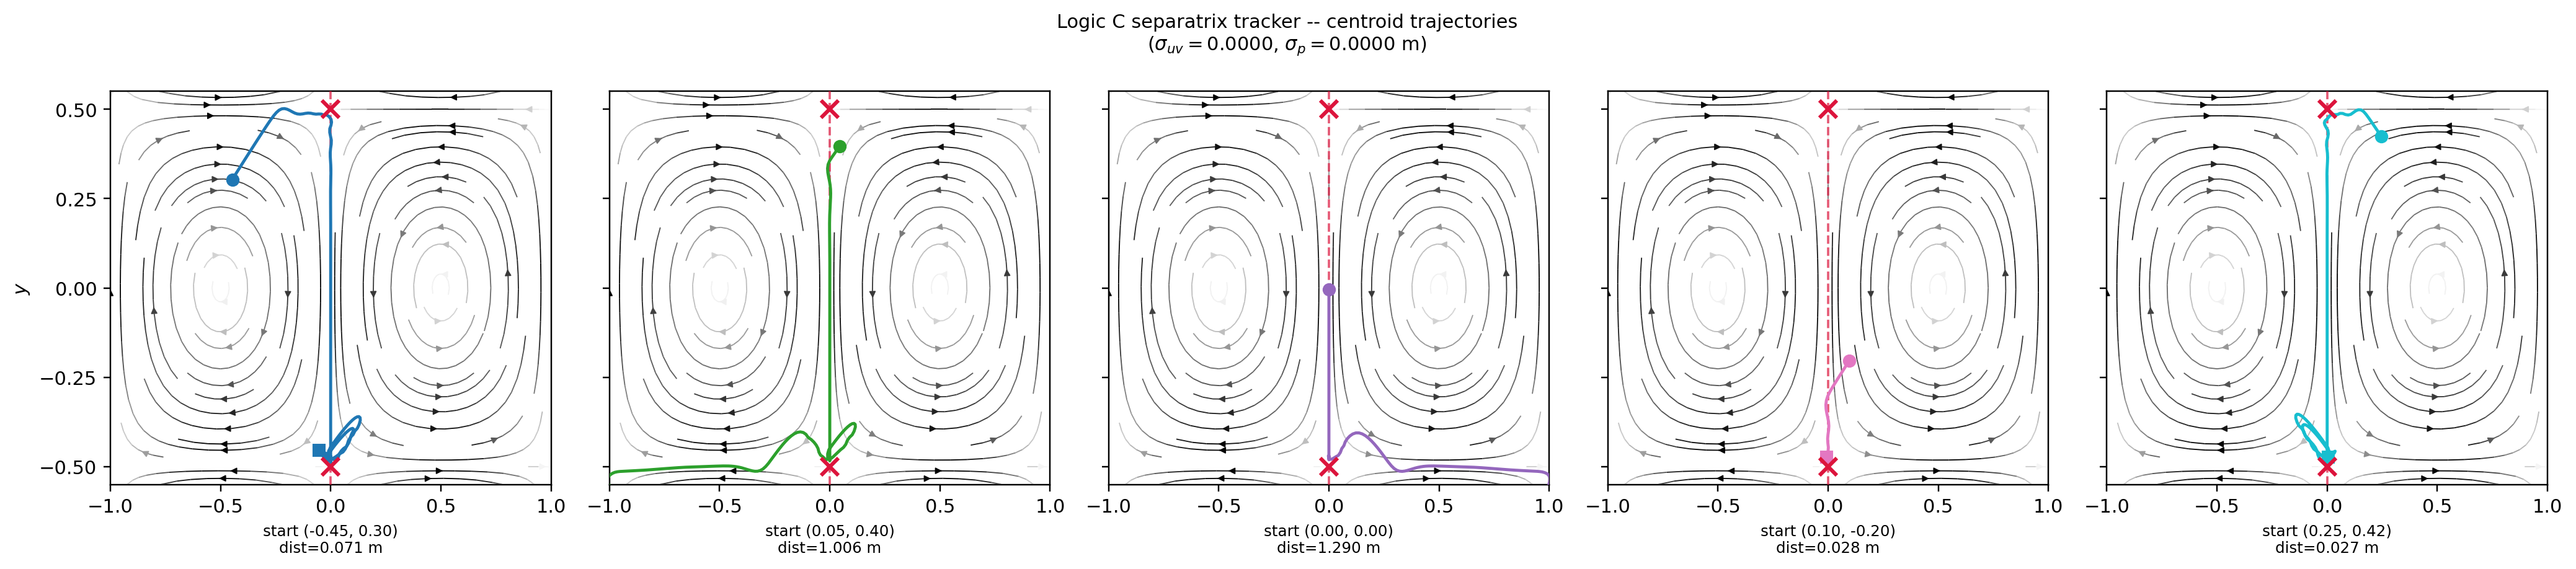
\includegraphics[width=0.34\textwidth]{figures/separatrix_trajectories.png}
    \caption{Noise-free $D$ tracker trajectories from six starts
    ($\bullet$), overlaid on the double-gyre streamlines and Okubo-Weiss
    diamonds. Every run reaches $x = 0$ and continues through the
    terminal saddle ($\times$) along the wall trench. Bottom: active
    selector-mode family (FLOW, SLIDE, ATTRACT) for each run versus
    control step.}
    \label{fig:sep_trajectories}
\end{figure}

From the six starts of Fig.~\ref{fig:sep_trajectories}, all six reach the
separatrix and pass within 0.02 of the bottom saddle
$\mathbf{p}^*_1$ (closest approach 0.0003--0.0194 across runs). The six
starts lie between $0$ and $2.7\rho$ from the nearest trench segment
($\rho = 0.075$, the formation radius): two begin within one $\rho$ of
the structure, consistent with their immediate banding, and the other
four start $1.1\rho$ to $2.7\rho$ off it; none of those four brackets
the separatrix at initialization. Two of
the six begin already inside the FLOW band and band immediately;
the other four take 6, 13, 18, and 35 steps. Mode occupancy over each run
is FLOW 6--37\%, SLIDE 34--48\%, and ATTRACT 10--24\%, with the
remainder in the flow-drift and attract-fallback refinements of the
same three modes. Every run continues past
the terminal saddle rather than stopping there. This traces to the
structural bias of $\hat{\mathbf{H}}_D$ (Section~\ref{sec:sensitivity}):
near the well the estimated eigenvalues are indefinite and more than an
order of magnitude too small, so the capture test
$\lambda_1\lambda_2 \geq 0$ of Section~\ref{sec:sep_controller} does not
fire even without noise. Section~\ref{sec:discussion} returns to this
behavior with terminal capture as a tightened-threshold special case.

\begin{table*}[!t]
\centering
\caption{Monte Carlo task success (\%): 10\,000 trials/cell from the
straddling start $(0, 0.35)$, random heading per trial, both scored
against the single far saddle $\mathbf{p}^*_1$ a noise-free ride from
this start reaches, over the full $\sigma_{uv} \times \sigma_p$ grid.
(a) $D$ tracker traverse success. (b) $s_1$ tracker traverse success;
the transition falls entirely between $\sigma_{uv} = 0.001$ and $0.005$
at every $\sigma_p$ shown, and at $\sigma_{uv} = 0$ entirely between
$\sigma_p = 0$ and $0.005$; both are resolved at 0.0005 spacing in
Fig.~\ref{fig:flip_resolution} and Section~\ref{sec:results_oecs}.}
\label{tab:mc_success}
\footnotesize
\setlength{\tabcolsep}{4pt}
\begin{tabular}{r|rrrrr}
\multicolumn{6}{l}{(a) $D$ tracker: traverse success (\%)} \\
\hline
$\sigma_{uv}$ \textbackslash\ $\sigma_p$ & 0.000 & 0.005 & 0.010 & 0.020 & 0.050 \\
\hline
0.000 & 100.0 & 65.7 & 44.5 & 33.3 & 19.0 \\
0.001 &  99.6 & 63.2 & 45.6 & 32.9 & 19.1 \\
0.005 &  62.4 & 52.1 & 43.5 & 31.2 & 19.4 \\
0.010 &  43.7 & 40.7 & 37.0 & 28.8 & 18.7 \\
0.020 &  25.5 & 25.7 & 24.3 & 22.6 & 17.0 \\
0.050 &  16.0 & 16.2 & 15.8 & 16.1 & 14.9 \\
0.100 &  14.1 & 14.1 & 14.3 & 14.6 & 13.6 \\
0.200 &  13.5 & 12.4 & 12.8 & 12.8 & 12.4 \\
0.400 &  12.1 & 12.2 & 12.0 & 12.3 & 11.9 \\
0.800 &   4.8 &  5.4 &  5.1 &  5.4 &  5.2 \\
\hline
\end{tabular}
\hspace{1.5em}
\begin{tabular}{r|rrrrr}
\multicolumn{6}{l}{(b) $s_1$ tracker: traverse success (\%)} \\
\hline
$\sigma_{uv}$ \textbackslash\ $\sigma_p$ & 0.000 & 0.005 & 0.010 & 0.020 & 0.050 \\
\hline
0.000 & 100.0 &  1.3 &  0.0 &  0.0 &  0.0 \\
0.001 &  91.8 &  1.1 &  0.0 &  0.0 &  0.1 \\
0.005 &   0.0 &  0.0 &  0.0 &  0.0 &  0.0 \\
0.010 &   0.0 &  0.0 &  0.0 &  0.0 &  0.0 \\
0.020 &   0.0 &  0.0 &  0.0 &  0.0 &  0.1 \\
0.050 &   0.2 &  0.2 &  0.1 &  0.1 &  0.1 \\
0.100 &   0.4 &  0.4 &  0.3 &  0.4 &  0.3 \\
0.200 &   0.5 &  0.4 &  0.5 &  0.4 &  0.4 \\
0.400 &   0.5 &  0.5 &  0.5 &  0.6 &  0.5 \\
0.800 &   0.5 &  0.6 &  0.4 &  0.6 &  0.4 \\
\hline
\end{tabular}
\end{table*}

Table~\ref{tab:mc_success}(a)'s traverse-success 50\% level, between
$\sigma_{uv} = 0.005$ and $0.01$ at $\sigma_p = 0$, coincides with the
open-loop $\nabla\hat{D}$ reliability threshold reported above: the
estimator, not the control law, sets the noise ceiling. Position noise
scales the same curve by $\|\mathbf{J}\|$, per the effective-noise
argument of Section~\ref{sec:sensitivity} ($\sigma_p = 0.01$ alone and
$\sigma_{uv} = 0.01$ alone give nearly identical rates), and beyond the
cliff success does not fall to zero but levels off in the low tens of
percent through $\sigma_{uv} = 0.2$, the unbiased-random-walk floor
that only decays at the extreme extension $\sigma_{uv} = 0.8$.
Straddle retention, the failure metric of \cite{9}, decays cleanly with
no such floor (1.000 at zero noise, 0.589 at $\sigma_{uv} = 0.005$,
0.389 at 0.01). Tracking error (mean $|x_c|$) rises from 0.002~m at
zero noise to 0.088~m at the cliff and saturates near 0.27~m. Binning
the 40\,000 trials at $\sigma_{uv} \leq 0.01$, $\sigma_p = 0$ by
initial-heading quartile gives 75.9--77.1\% success per quartile,
confirming the isotropy of Lemma~\ref{lem:gains}.

Acquisition from off-structure starts was swept over the same noise
grid at $\sigma_p \in \{0, 0.01\}$, 1000 trials per cell, from the two
clean-run starts $2.7\rho$ off the structure: the weak-strain start
near the left gyre center and the strain-region start in its lower
half. The team reached the trench network, closest approach under
0.05, in every one of the 20\,000 trials through $\sigma_{uv} = 0.02$
and in at least 97.5\% at $\sigma_{uv} = 0.05$: acquisition of the
trench network itself is not the noise-limited phase. Arrival at the
one designated terminal saddle is a different quantity, set by which
branch of the network the descent reaches first, not by noise
(Section~\ref{sec:limitations}). From the gyre-center start, whose
ride takes the south branch at $\mathbf{p}^*_2$, arrival holds near
40\% from zero noise through $\sigma_{uv} = 0.01$ and drops sharply
between $\sigma_{uv} = 0.01$ and $0.02$, one grid step later than the
straddling start's own cliff in Table~\ref{tab:mc_success}(a). The
strain-region start feeds the bottom wall, whose flow leads away from
$\mathbf{p}^*_1$, and arrives only through the direct path: 24.1\% at
exactly zero noise, near zero under any perturbation.

\subsection{Double Gyre: The $s_1$ Tracker}
\label{sec:results_oecs}

\subsubsection{Noise-free runs}
From the same six starts used for the $D$ tracker's own traverse
(Fig.~\ref{fig:sep_trajectories}), spanning both gyre halves, the
origin, and points off the structure entirely, the $s_1$ tracker
acquires the trench (time-to-band 0 to 46 steps, longest from the
farthest off-structure start) and rides it through the eigenvector swap
at the origin with no dedicated crossing behavior: over the sweep of
$r_{\text{band}}$ from 0.05 to 0 reported in
Section~\ref{sec:limitations}, CROSS never fires once, so the crossing
is carried entirely by ordinary tangent selection
(\ref{eq:tangent_select}). All six starts reach CAPTURE, at whichever
saddle their initial tangent orientation resolves toward: three end
within 0.02 of $\mathbf{p}^*_2 = (0, 0.5)$, three at $\mathbf{p}^*_1 = (0, -0.5)$. The mean
path gap against the $D$ tracker's own trajectory from the same start,
measured over the common on-trench portion of each run, is 0.02 to 0.32
across the six, growing only where the two controllers commit to
different saddles from a start equidistant enough that the flow-seeded
tangent and the $D$ tracker's own flow-tested FLOW step do not agree;
where they commit to the same saddle the two paths are visually
coincident until the $s_1$ tracker settles and the $D$ tracker continues
onto the crossing wall trench, the divergence Remark~\ref{rem:capture_gap}
already predicts for the $D$ tracker's own selector. This is the
designed contrast with Fig.~\ref{fig:sep_trajectories}: both controllers
traverse the same network from the same objective starting condition,
but only the $s_1$ tracker's capture test is built to fire reliably at
what it finds.

\begin{figure}[!t]
    \centering
    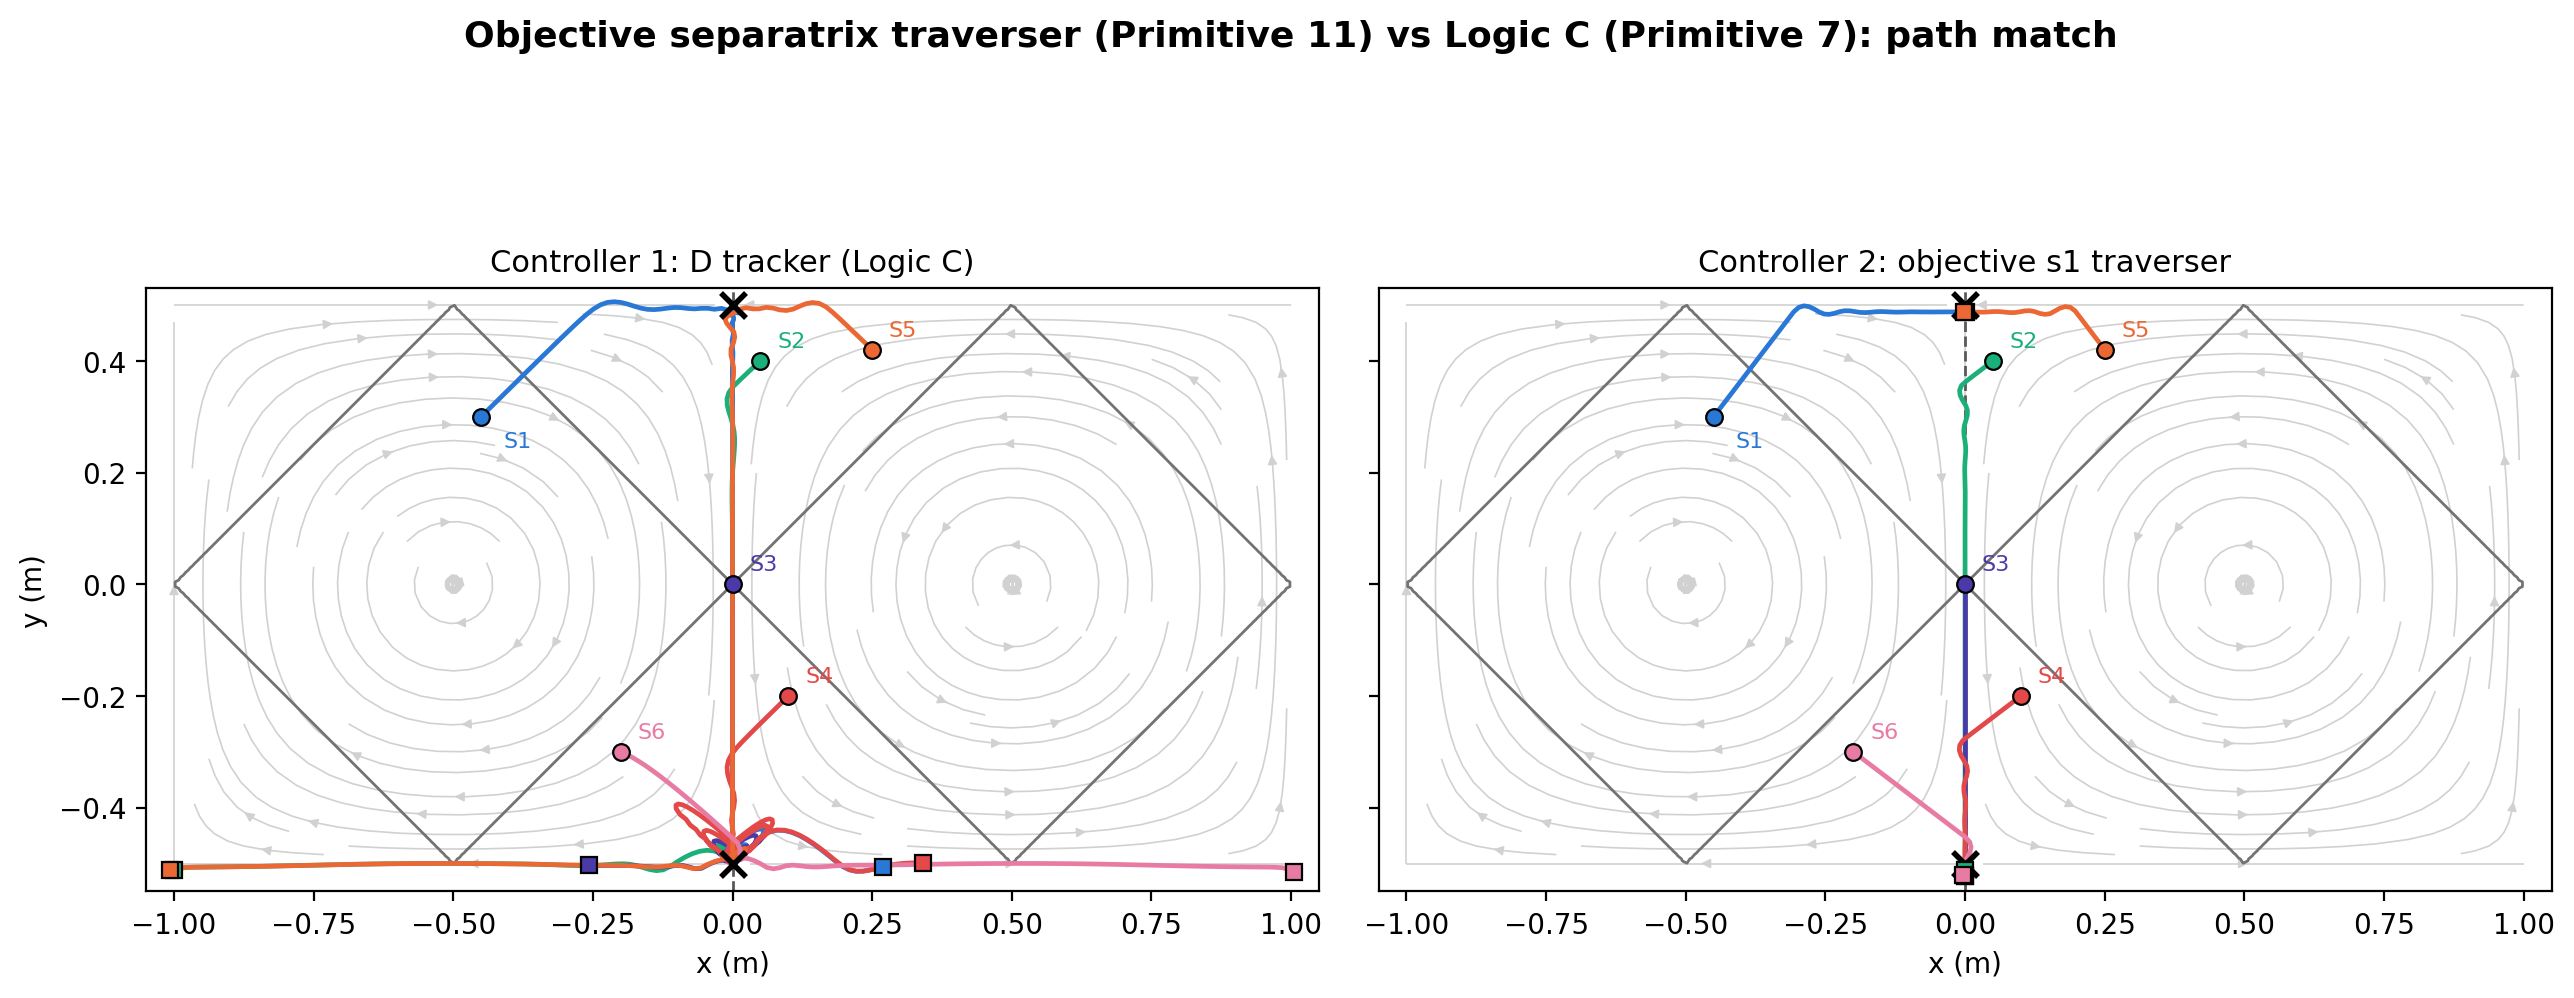
\includegraphics[width=0.34\textwidth]{figures/traverse_vs_logic_c.png}
    \caption{$s_1$ tracker versus $D$ tracker, six matched starts,
    noise-free. Both traverse the same network through the eigenvector
    swap at the origin; the $s_1$ tracker captures at the nearest saddle
    its tangent orientation resolves toward, while the $D$ tracker
    continues onto the crossing wall trench past every saddle it
    reaches.}
    \label{fig:traverse_vs_logic_c}
\end{figure}

\subsubsection{Objectivity}
The objectivity demonstration follows the rotating-frame protocol of
Section~\ref{sec:test_plan}. Fig.~\ref{fig:oecs_objectivity} shows the
outcome. The $s_1$ tracker's two runs are the same material path: final
gap 0.025, mean gap 0.014 over the common steps, with mean distance to
the true trench network of 0.000 (inertial) and 0.005 (rotating); both
runs traverse the same eigenvector swap and capture at the same bottom
saddle. The $D$ tracker's two runs are not: the rotating observer's $D'$
landscape (\ref{eq:D_not_objective}) and swirl-contaminated flow
measurement carry the team off the separatrix entirely, to a mean
trench-network distance of 0.052 (ten times its inertial value of
0.005) and a final gap of 1.219 from its inertial twin, ending in the
gyre interior where no structure exists. Under a rotating observer the
$D$ tracker follows a frame artifact; the $\mathbf{S}$-based tracker
does not, past the single seeding instant Proposition~\ref{prop:equivariance}
identifies, and unlike an intermediate design that selected
(\ref{eq:tangent_select}) by projection onto the flow at every step
rather than the gradient, which was found to inherit exactly this
artifact at every step, not only at the seed (verified: final gap 1.06
at the same $\Omega$, tracking the true structure closely in both frames
yet still committing to different branches from it), the gradient-only
rule confines the frame dependence to that one instant rather than
carrying it for the life of the run.

\begin{figure}[!t]
    \centering
    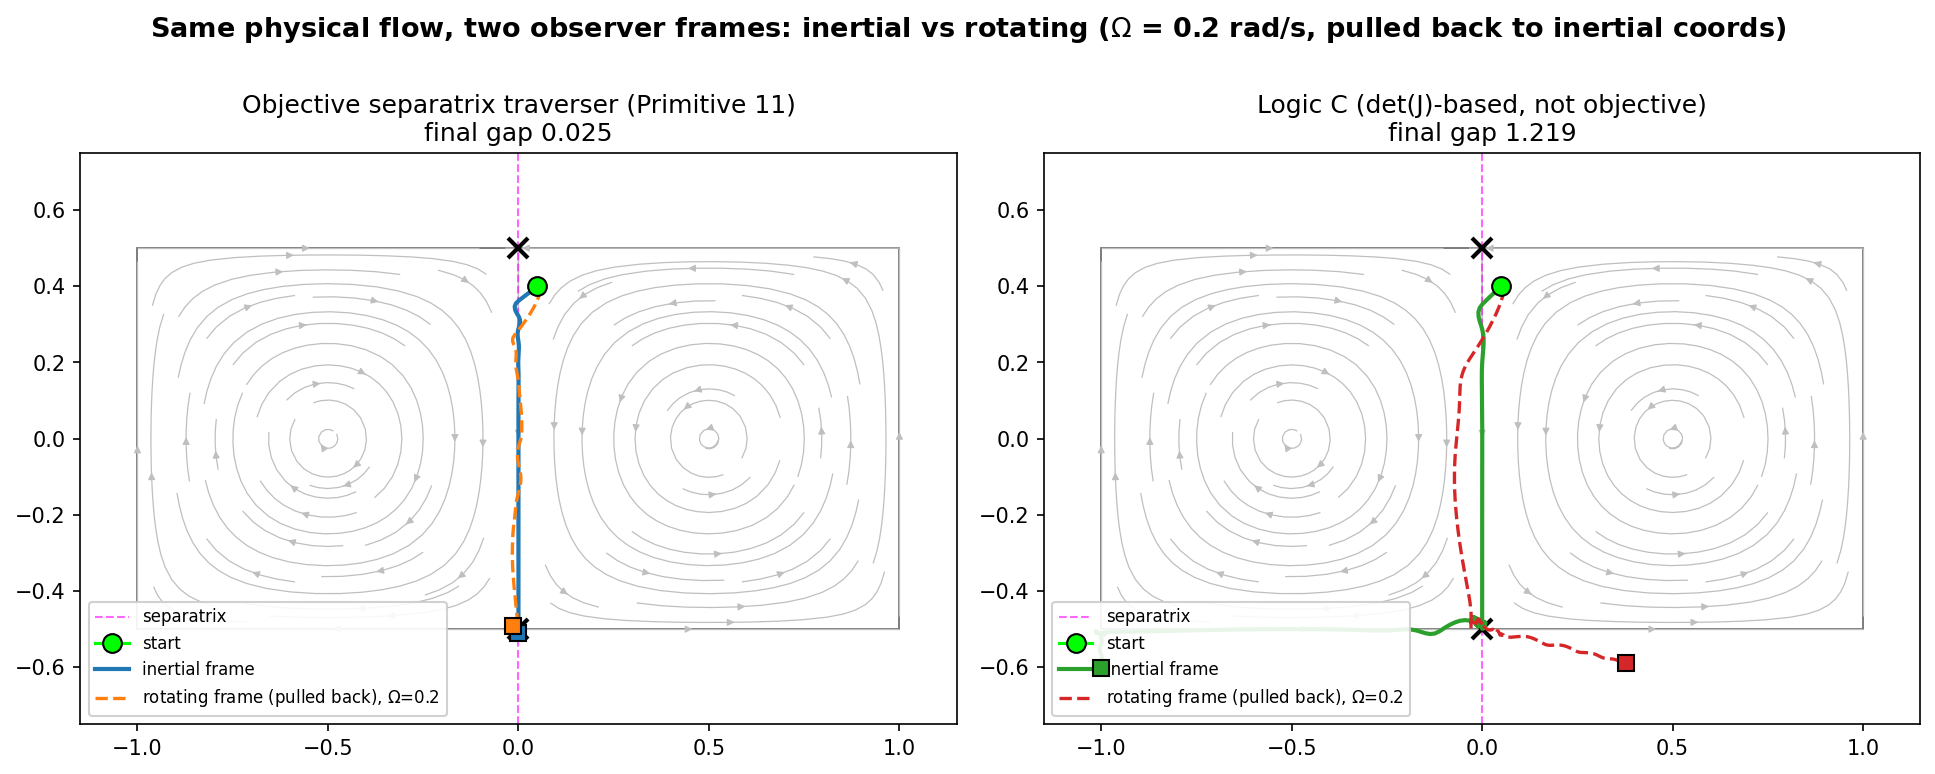
\includegraphics[width=0.38\textwidth]{figures/oecs_objectivity.png}
    \caption{Objectivity experiment: each controller run in the
    inertial frame (solid) and in a frame rotating at $\Omega = 0.2$
    rad/s (dashed, pulled back to inertial coordinates). Left: the
    $s_1$ tracker's trajectories coincide (final gap 0.025). Right: the
    $D$ tracker's rotating-frame run leaves the separatrix (final gap
    1.219), the artifact predicted by (\ref{eq:D_not_objective}).}
    \label{fig:oecs_objectivity}
\end{figure}

\subsubsection{Noise robustness}
Table~\ref{tab:mc_success}(b) reports traverse success for the $s_1$
tracker over the same noise grid, scored against $\mathbf{p}^*_1$
specifically rather than either saddle: the flow-seeded tangent
orientation (\ref{eq:tangent_select}) at this start can commit to
either, and only contact with the same saddle a noise-free ride
reaches counts as riding the separatrix rather than substituting an
easier, shorter task. The zero-noise tracking error is 0.0075, about
five times the $D$ tracker's 0.0016, the gradient-rate cost predicted
by Remark~\ref{rem:s1hess}. Under noise the two controllers do not
degrade the same way. Fig.~\ref{fig:flip_resolution} resolves the
transition at 0.0005 spacing: success falls from 91.8\% at
$\sigma_{uv} = 0.001$ through 43.6\% at 0.002 to 6.7\% at 0.003, a
smooth decline over one decade of noise, not a discontinuity at a
single value, and by $\sigma_{uv} = 0.005$ it has reached the
random-walk floor it holds out to 0.008 (under 1\% throughout). This is
markedly steeper than the $D$ tracker's own curve, whose corresponding
column falls from 62.4\% only to 43.7\% across the same
$\sigma_{uv} = 0.005$--$0.01$ span: the $D$ tracker degrades gradually
at a fixed target, while the $s_1$ tracker's target itself becomes
unreliable well before its own transverse regulation would predict
failure. The mechanism is the one-time flow read
(Section~\ref{sec:oecs_controller}) that seeds $\mathbf{t}_{\text{ref}}$
on the first tracking step: at this start the differential flow signal
across the six sample points is small (span $\approx 0.12$~m/s),
comparable to $\sigma_{uv}$ in the 0.001--0.003 range, so the sign the read
resolves becomes an even bet well before the transverse channel's own
noise tolerance is exceeded. Because the decision is made once, not
accumulated over the ride, its failure looks like a step in success
rather than a gradual drift in tracking error.

Table~\ref{tab:mc_success}(b) shows the same collapse along the
$\sigma_p$ axis at $\sigma_{uv} = 0$ (100.0\% at $\sigma_p = 0$, 1.3\%
already by $\sigma_p = 0.005$) with no points between to show its
shape; Fig.~\ref{fig:flip_resolution}(b) resolves it at the same
0.0005 spacing, 10\,000 trials/cell. The curve is the same smooth
decline as panel (a), not a sharper cliff: success falls from 99.8\%
at $\sigma_p = 0.0005$ through 63.6\% at 0.002 to 6.6\% at 0.004,
crossing 50\% between $\sigma_p = 0.002$ and 0.0025, close to panel
(a)'s own $\sigma_{uv}$ crossing. This is the mechanism already
identified for the $D$ tracker (Section~\ref{sec:results_sep}):
position noise enters through the same effective-measurement-error
coupling $\mathbf{J}(\mathbf{p}_i)\boldsymbol{\xi}_i$ of
(\ref{eq:pos_noise}), so at this test point, where the $D$ tracker's
own noise grid gave $\|\mathbf{J}\| \approx 1$, a given $\sigma_p$
degrades the tangent-sign read by roughly the same amount as an equal
$\sigma_{uv}$ would. The two panels are one finding measured on two
axes, not two separate failure modes: whichever noise channel is
active, it is the one-time flow read that fails first, well before
the transverse channel's own regulation would predict trouble.

Straddle retention, conditioned on the same $\mathbf{p}^*_1$ contact
(a trial that stops at the wrong saddle has no straddle-to-$\mathbf{p}^*_1$
history to report), stays below success at every level shown
(73.2\% against 91.8\% at $\sigma_{uv} = 0.001$, 47.6\% against 71.5\%
at 0.0015, reaching zero by 0.004 where success itself is already under
1\%), consistent with straddle being the stricter condition once both
are scored against the same target. The $D$ tracker's own straddle
retention decays more gradually over the same interval (0.589 at 0.005,
0.389 at 0.01) and does not depend on which saddle is reached, since its
target never moves.

The tangent-selection mechanism itself
(\ref{eq:tangent_select}) is not the source of this fragility: it uses
only the already-computed gradient projections, and
Section~\ref{sec:s1_estimation}'s result that the tangent direction
survives noise past the point every gradient-based quantity approaches
chance still applies to whichever eigenvector it currently selects. The
fragility is specific to the sign convention at the seed, a single
comparison against the ambient flow, and Section~\ref{sec:limitations}
returns to whether a start-independent alternative is worth adopting.

\begin{figure*}[!t]
    \centering
    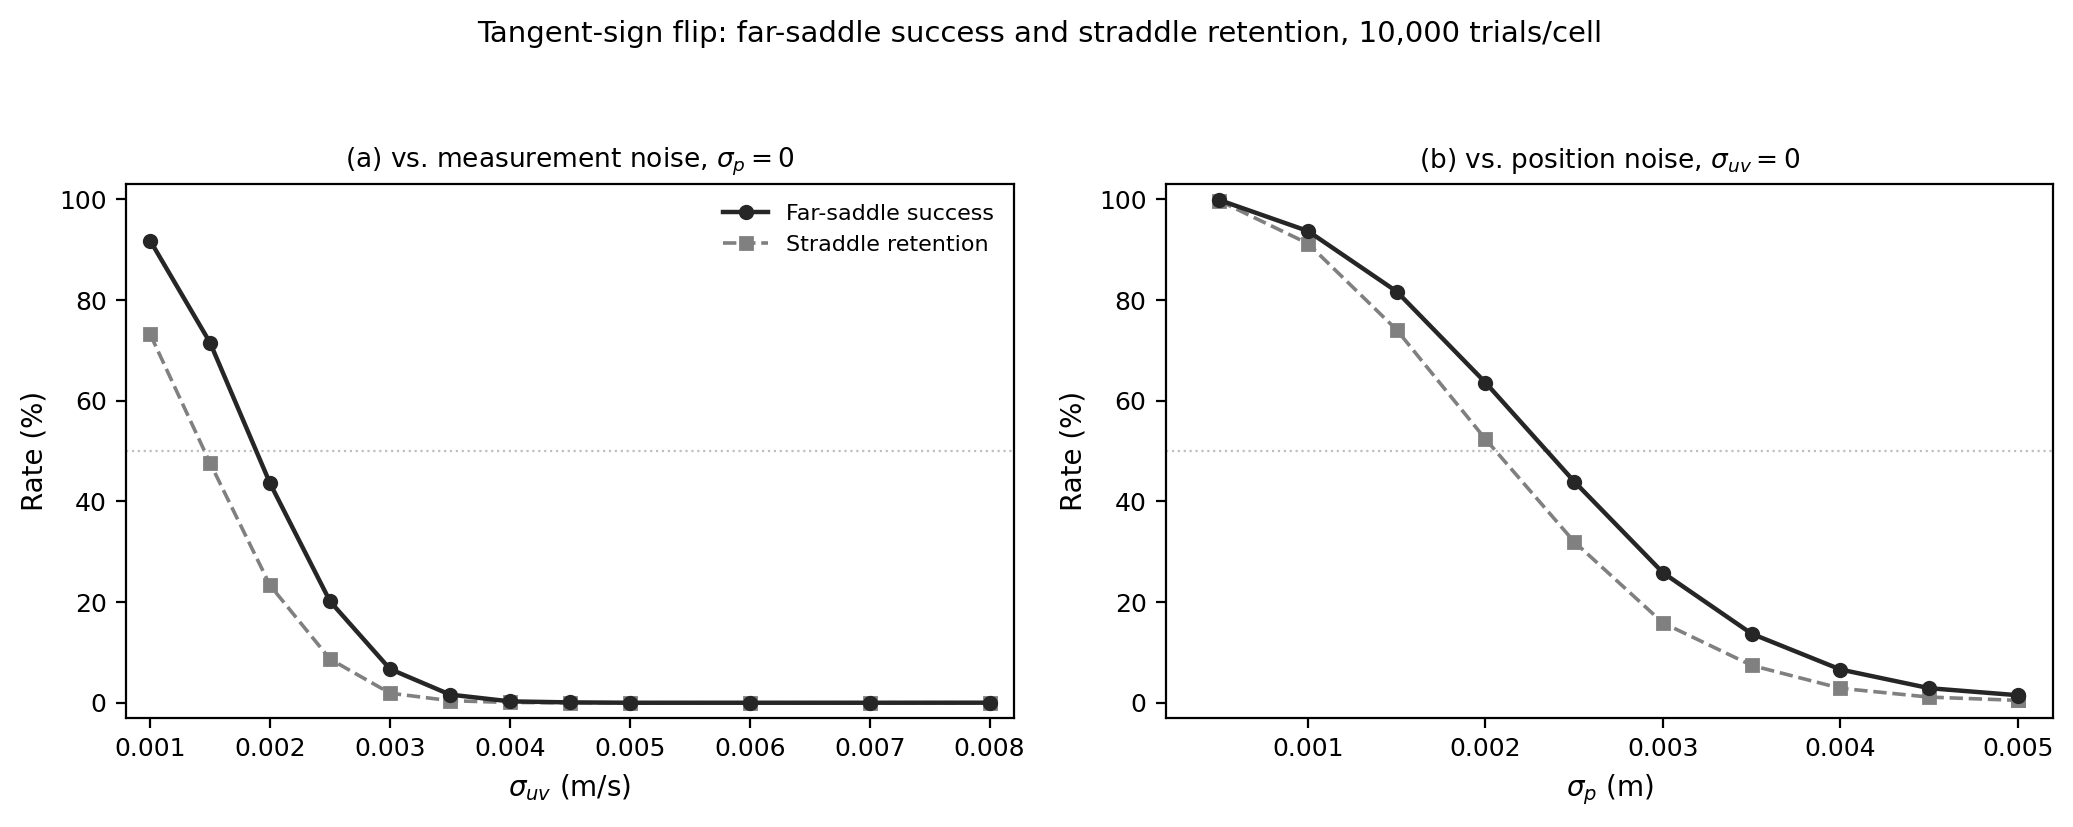
\includegraphics[width=0.78\textwidth]{figures/flip_resolution.png}
    \caption{Resolving the tangent-sign flip: far-saddle success and
    straddle retention (both conditioned on reaching $\mathbf{p}^*_1$),
    10\,000 trials/cell, at 0.0005 spacing on each axis. (a) Against
    $\sigma_{uv}$, $\sigma_p = 0$: success crosses 50\% between
    $\sigma_{uv} = 0.0015$ and 0.002 and reaches a sub-1\% floor by
    0.005, held out to 0.008. (b) Against $\sigma_p$, $\sigma_{uv} = 0$:
    the same smooth decline, crossing 50\% between $\sigma_p = 0.002$
    and 0.0025. Neither panel shows a discontinuity.}
    \label{fig:flip_resolution}
\end{figure*}

Open-loop checks at the nominal radius confirm the structural picture
behind these margins. The fitted shear strain at three test points is
at the $10^{-4}$ level (analytic value zero); the fitted
$\hat{\mathbf{H}}_{s_1}$ eigenvalues are $[-0.011, 0.000]$ and smaller,
negative semidefinite as Remark~\ref{rem:s1hess} requires; the
transverse component of (\ref{eq:grad_s1}) recovers the restoring slope
$4.0$ per unit offset; and at $\sigma_{uv} = 0.01$ the median direction
error of $\mathbf{e}_2$ is $4.5^\circ$, against $44^\circ$ for
$\nabla\hat{s}_1$ and $41^\circ$ for the $\hat{\mathbf{H}}_D$
eigenvector ($2\times 10^4$ draws per level).

\subsection{Ocean HFR: The $D$ Tracker}
\label{sec:results_ocean}

The $D$ tracker was run from a single start north of the channel
entrance, $(34.40^{\circ}\mathrm{N}, -120.39^{\circ}\mathrm{W})$, at
the operating point of Table~\ref{tab:params}. Over the 28~h trial the
cluster descends through the channel entrance, tracks the ridge through
the bifurcation, and continues to landfall on the middle island's north
coast.
Fig.~\ref{fig:ocean_ftle}
places the trial against the 24-h forward-time FTLE field, computed
offline over the same window in the style of \cite{17}; the cluster's path
follows the dominant FTLE ridge running from the channel entrance to the
bifurcation closely, without the ridge being available to the controller
at any point, only the local $\hat{D}$ and $\hat{\mathbf{g}}$ estimates
that Section~\ref{sec:estimation} builds from the current samples at the
formation.

\begin{figure}[!t]
    \centering
    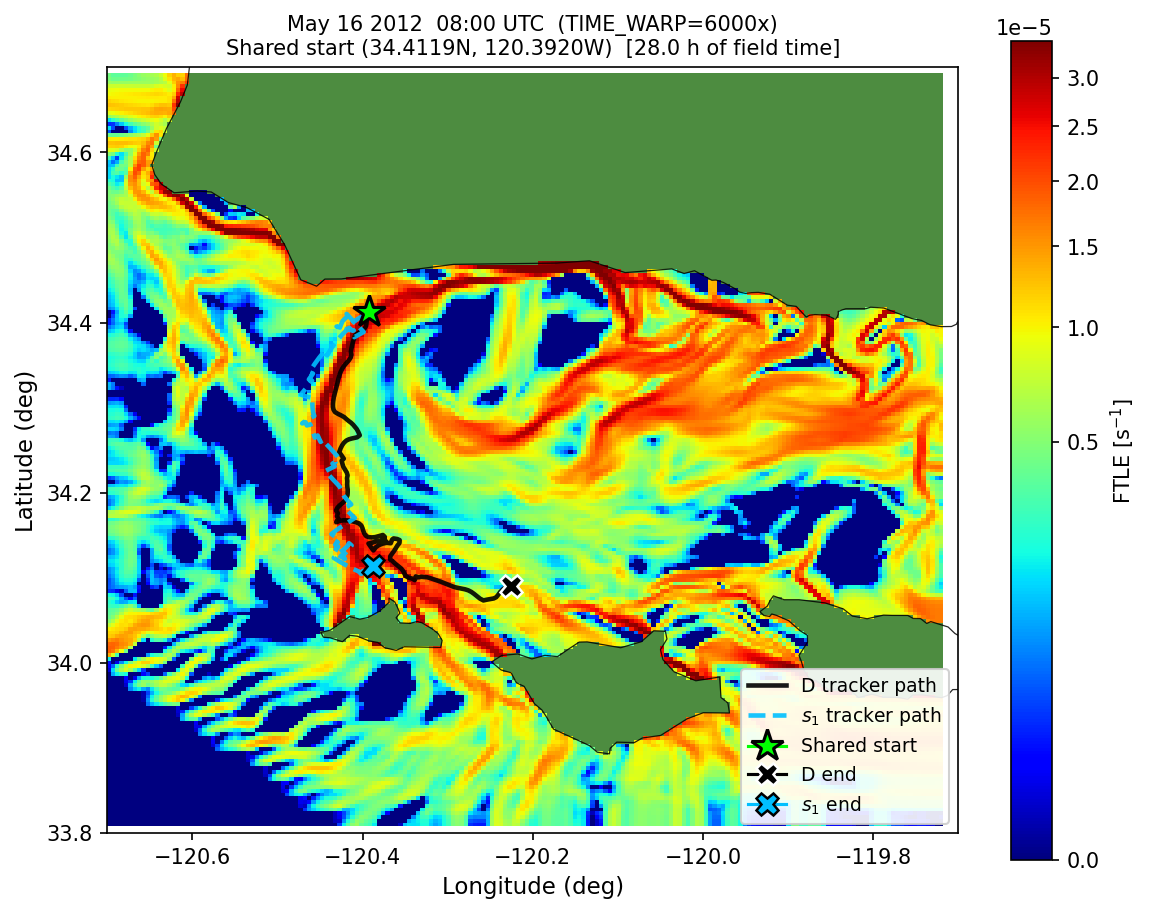
\includegraphics[width=0.38\textwidth]{figures/ocean_ftle_trajectory_overlay_2km.png}
    \caption{28-h $D$ tracker path over the 24-h forward FTLE field
    computed offline from the same 2~km data. The path follows the
    dominant ridge from the channel entrance to landfall.}
    \label{fig:ocean_ftle}
\end{figure}

Forward FTLE recomputed at four anchor times across the record (0, 5,
10, and 16~h, each integrated 12~h forward) confirms that the dominant
ridge persists while the finer structure downstream evolves: the
experiment is genuinely time-varying, and the controller sees only the
instantaneous samples at its own formation position.

A $10 \times 10$ grid of starts jittered $\pm 0.05^{\circ}$ around the
validated start tests sensitivity to the initial condition. Of the 100
starts, 84 land on the same middle-island branch as the validated
trial; the remaining 16, all on or within one grid cell of the
jitter-box edges furthest from the ridge, are carried onto a western
branch that does not make landfall in the domain. This is a
basin-of-attraction result in the sense of
Section~\ref{sec:limitations}, not a robustness guarantee: the tracked
branch is the typical outcome for starts near the validated one, not
the destination of every start.

\subsection{Ocean HFR: The $s_1$ Tracker}
\label{sec:results_ocean_oecs}
The $s_1$ tracker was run on the real 2~km field at the operating point
of Table~\ref{tab:params}, $s_{\text{capture}}$ unset so the team
relies on CAPTURE alone. Started at the $D$ tracker's own initial
condition, the team locks onto a local structure near the channel
entrance and holds it for the full record without traveling; a second
run, started instead at $(34.26^{\circ}\mathrm{N},
-120.42^{\circ}\mathrm{W})$, a point on the $D$ tracker's own ridge
roughly 8~h into its run, is reported here for the traverse it produces.
Ground truth is computed offline from the full radar grid in the style
of \cite{17,36}, TRAP cores as local minima of $s_1$ at each hourly
frame; unlike the double gyre, the ocean strain field is generic, with
isolated degeneracies and cores that move between frames, so this
experiment also exercises tangent selection (\ref{eq:tangent_select}) on
a live field where neither the eigenframe nor the trench network is
axis-aligned. Fig.~\ref{fig:ocean_oecs} shows the outcome: over the full
28-h record the team stays in TRACK mode throughout, riding the ridge
network southeast across the channel, crossing structure the $D$
tracker's own path also crosses before continuing past it, and ends
$11.1$~km from the nearest of 92 TRAP cores extracted offline from the
full radar grid at the final frame. A genuine two-dimensional minimum of
$s_1$ was never reached (CAPTURE does not fire; the team rides the ridge
through ordinary transverse and tangential regulation throughout), so
the terminal mean $\hat{s}_1$ along the ride, $-0.66$, is the tracked
value rather than a certified capture, a legitimate outcome of the same
selector, not a failure of it: on this field, absent a stationary point
of $s_1$ close enough to the ride to trigger CAPTURE, the $s_1$ tracker
behaves as a traverser, reading the same ridge structure the $D$ tracker
does from the objective strain term alone. Which segment of the network
the ride commits to, like the choice of which saddle to capture at on
the double gyre, is set by where the ride's tangent orientation is first
resolved relative to the local flow, not by proximity to the strongest
structure in the domain; the run from the $D$ tracker's own start does
not reach far enough from that structure for this to matter; the second
run does.

\begin{figure}[!t]
    \centering
    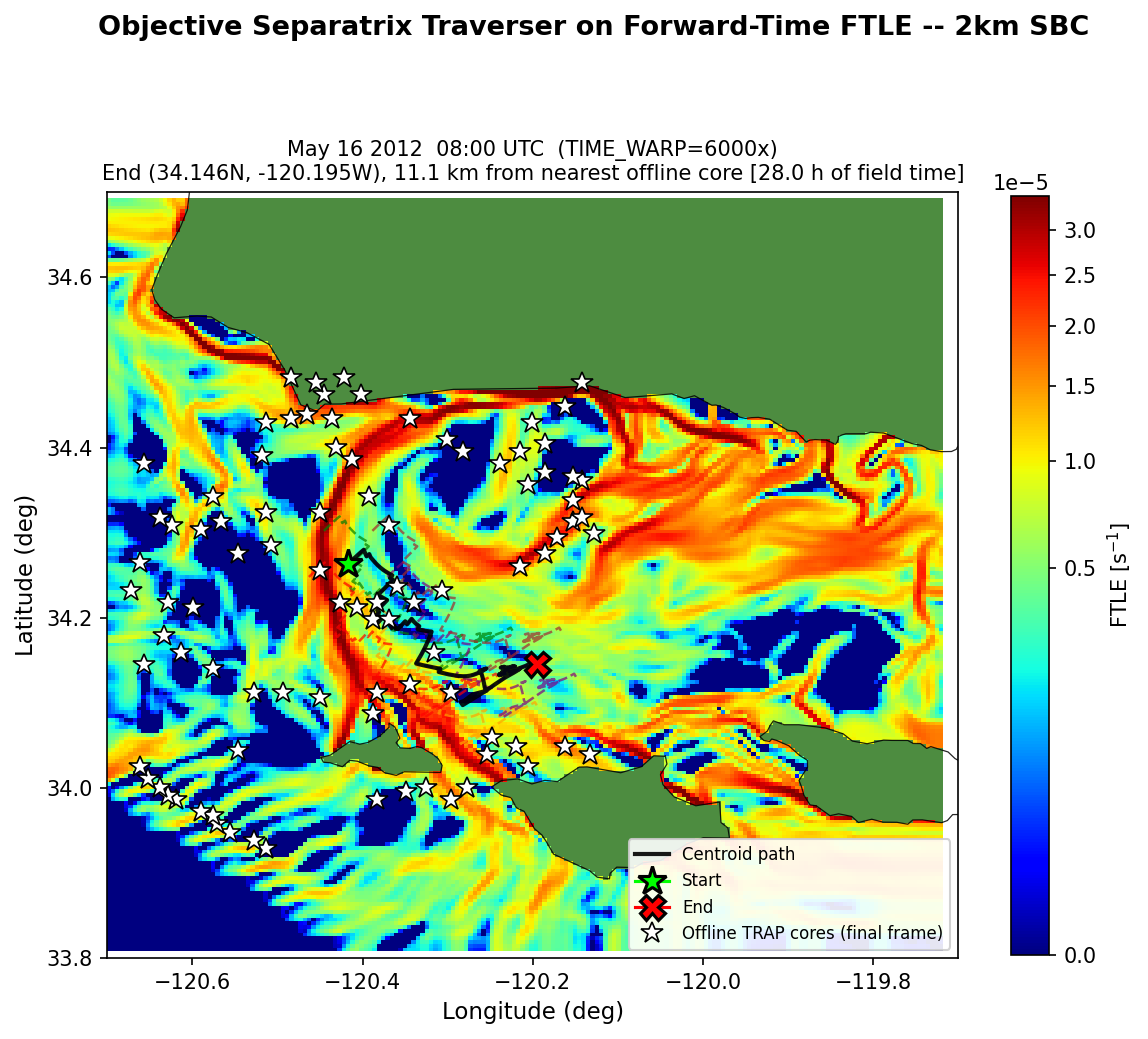
\includegraphics[width=0.38\textwidth]{figures/traverse_trajectory_overlay_2km.png}
    \caption{$s_1$ tracker on the 2~km Santa Barbara Channel field,
    started at $(34.26^{\circ}\mathrm{N}, -120.42^{\circ}\mathrm{W})$, a
    point on the $D$ tracker's own ridge. The team rides the ridge
    network southeast for the 28-h record, crossing structure the $D$
    tracker's own path also crosses, and ends 11.1~km from the nearest
    of 92 offline TRAP cores (white stars).}
    \label{fig:ocean_oecs}
\end{figure}

\section{Discussion}
\label{sec:discussion}

\subsection{Implications}
\label{sec:prior_comparison}

Tracking a trench is structurally harder than tracking a regular level
set: a level set is fixed by first-order information, while the trench
lives exactly where that gradient vanishes in the normal direction, so
controller and proof alike must synthesize the missing direction from
curvature, the price paid by the eigenstructure dependence, mode
switching, and tube assumptions of Section~\ref{sec:stability}. Against
the straddle family \cite{9,10,11} (Section~\ref{sec:related_robots}),
the method here additionally solves acquisition and traversal from
starts off the structure, within the basin
Section~\ref{sec:limitations} maps (Fig.~\ref{fig:basin_map}), and
resolves branch identity at each crossing from the current fit; the two
problem statements do not coincide, and a controlled head-to-head on
identical fields, formations, and noise is future work.

\subsection{Park versus Traverse}
\label{sec:park_vs_traverse}

Remark~\ref{rem:capture_gap} identifies the terminal-capture test as
the reason the deployed controller continues through every saddle: the
biased $\hat{\mathbf{H}}_D$ makes it unreliable exactly where it would
need to fire. An estimator-aware alternative restores capture using
only the two quantities free of the Hessian's structural bias,
$\hat{D}$ and $\hat{\mathbf{g}}$: the \emph{park step}, a fourth
case checked before the FLOW test in (\ref{eq:d_selector}),
\begin{equation}
    \dot{\mathbf{p}}_c =
    -\mathrm{sat}(\hat{\mathbf{g}})
    \quad \text{if } \hat{D} < D_{\text{capture}},
    \label{eq:park_step}
\end{equation}
componentwise saturated gradient descent on $\hat{D}$, which carries
its own certificate: with exact estimates $D$ itself is the Lyapunov
function ($\dot{D} = -\sum_k g_k\,\mathrm{sat}(g_k) \leq 0$), so the
team settles at the nearest local minimum of $D$, the flow saddle at
the end of the current trench segment. $D_{\text{capture}}$ is the
one-parameter knob: $D_{\text{capture}} = -\infty$ disables the test
and the controller is trajectory-identical to the base selector
(verified bit-exact in simulation), while a finite threshold inside the
well (here $-0.5$, roughly half the well depth $\pi^4 A^2 \approx
0.974$) parks the team there. Fig.~\ref{fig:park_vs_traverse} runs both
settings from the same start, noise-free: traverse exits the domain
after 228 steps riding the crossing trench; park settles 0.0124~m from
$\mathbf{p}^*_1$ with zero position drift over its final 100 steps. One
threshold thus recovers whichever behavior a mission calls for,
terminal parking at a critical point or open-ended traversal of the
network.

\begin{figure}[!t]
    \centering
    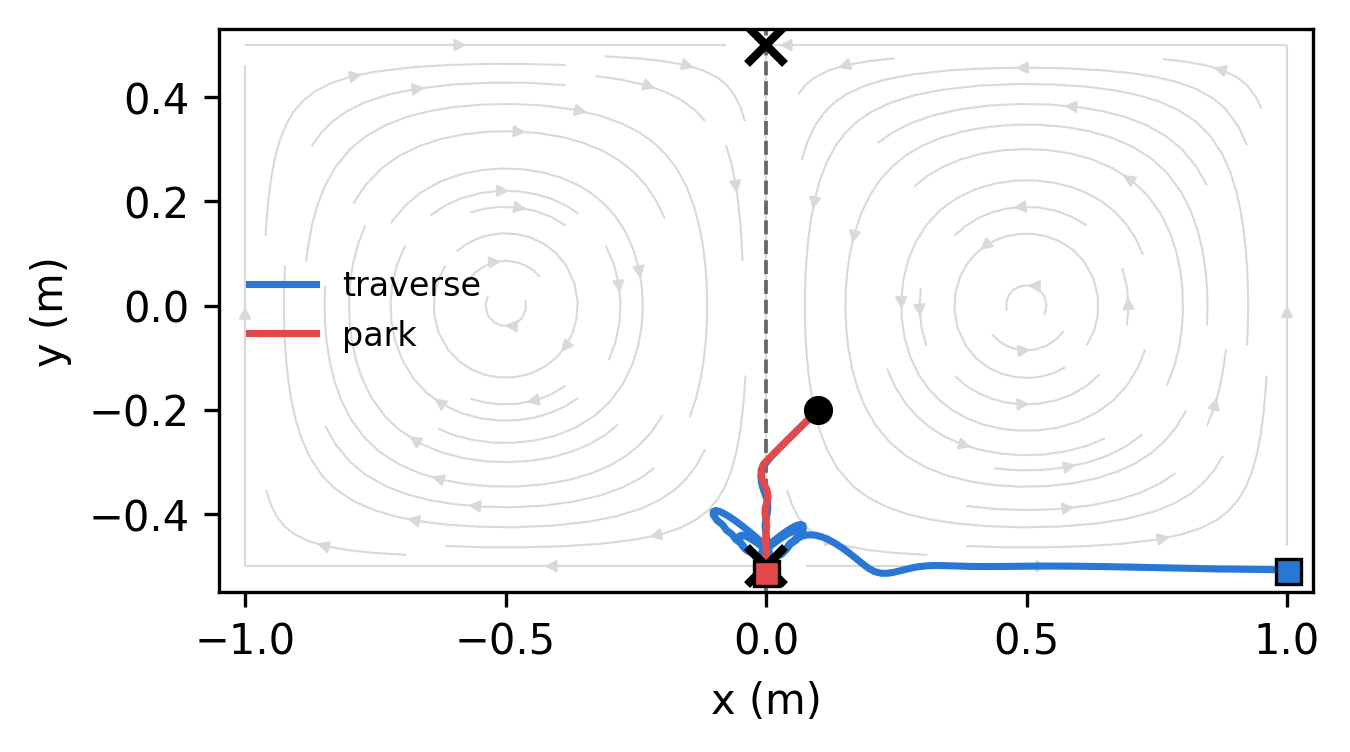
\includegraphics[width=0.33\textwidth]{figures/park_vs_traverse.png}
    \caption{Park versus traverse from the same start, noise-free.
    Traverse (the default selector) rides the trench through the bottom
    saddle and exits the domain; park ($D_{\text{capture}} = -0.5$)
    holds the team 0.0124~m from the saddle.}
    \label{fig:park_vs_traverse}
\end{figure}

\subsection{Objectivity Tradeoffs}
\label{sec:objectivity_tradeoff}

The two controllers are the two sides of the tradeoff carried by
(\ref{eq:splitting}), and Fig.~\ref{fig:oecs_objectivity} makes the
price concrete: a platform whose navigation frame turns relative to
the Earth inflates $\omega^2/4$ (\ref{eq:D_not_objective}), moving the
$D$ tracker's trench and contaminating its flow-tested selector, while
the $s_1$ tracker's strain-only pipeline, including tangent selection
(\ref{eq:tangent_select}), stays on the true material curve past the
single seeding instant. Zero-noise reach costs nothing on the double
gyre, where the two trenches coincide exactly; what it costs there is
rate (gradient- rather than Newton-normalized transverse convergence,
0.0075 zero-noise tracking error against 0.0016) and, under noise, the
tangent's one-time flow-seeded sign committing to the wrong end of the
network well before the transverse channel itself degrades
(Section~\ref{sec:results_oecs}). On the ocean field, where no
stationary point of $s_1$ sits near the ride,
Section~\ref{sec:results_ocean_oecs} shows the $s_1$ tracker traversing
rather than capturing, the same behavior the $D$ tracker shows
everywhere. A mission whose separatrix carries vorticity, or whose
platform is fixed in a known frame, may prefer the $D$ tracker's Newton
rate and more reliably determined target; one that needs frame-proof
material prediction, or operates from a rotating or drifting platform,
gains that guarantee at the cost this section quantifies. Both consume
the same fit, so the selection is one function call, not a new
estimator or formation.

\subsection{Failure Modes}

Three behaviors fall outside the guarantees of
Section~\ref{sec:stability}. First, the estimator is ill-conditioned
whenever the six sampling points drift toward a common conic
(Proposition~\ref{prop:conic}); monitoring $\det(\boldsymbol{\Phi})$
and adding a shape-maintenance term is the direct mitigation (the
Monte Carlo collapse flag, RMS inter-robot distance error above 0.30,
never triggers in any reported trial). Second, noise can chatter the
$D$ tracker across the FLOW-band boundary (\ref{eq:flow_band}); since
every mode shares the transverse dynamics (\ref{eq:n_dynamics}),
chatter costs only along-trench speed, and $\varepsilon_{\text{dim}}$
trades this against the crest stall of Section~\ref{sec:dg_example}
(fixed once at 0.025, never retuned).

Third, the $s_1$ eigenframe is noise-fragile where $\mathbf{S}$
approaches isotropy, a property of the physics rather than the
estimator (angular error scales as coefficient noise over the
eigenvalue gap $2r$, singular at the tensor lines themselves,
Section~\ref{sec:strain_field}). Before banding, $r_{\text{band}}$
hands such a region to ACQUIRE (or, first step only, CROSS), both
gradient-only; once tracking is underway, tangent selection
(\ref{eq:tangent_select}) is the primary defense, comparing gradient
alignment rather than trusting either eigenvector's identity, with
continuity fixing only the residual sign. The residual risk, a wrong
branch at a genuine crossing under heavy noise, is not fully excluded
by CAPTURE's gradient-magnitude test either, since noise can
transiently pass or fail it near but not at the true well; the bounded
latch (released once $\hat{s}_1$ rises back above $-s_{\text{trim}}$)
damps this without excluding it, and the generic ocean field exercises
the whole mechanism directly.

\subsection{Limitations}
\label{sec:limitations}

The $s_1$ tracker's tangent sign, resolved once from the ambient flow
at the first tracking step (Section~\ref{sec:oecs_controller}), is only
as reliable as the local differential flow signal is large relative to
the noise level; at the straddling start of Table~\ref{tab:mc_success}(b)
that signal is weak enough that the resolved sign becomes an even bet
by $\sigma_{uv} = 0.002$ (Fig.~\ref{fig:flip_resolution}). Three
unimplemented alternatives trade this differently: a start-independent
convention (e.g., a fixed world-axis component of $\mathbf{e}_2$)
removes the flow dependence at the cost of an arbitrary discontinuity,
the same kind CROSS's own flow-only fallback already accepts; a
confidence check on the seed converts a wrong commitment into a longer
ACQUIRE phase at the cost of a noise-level estimate the controller does
not otherwise need; and re-fitting the sign over several early steps
trades the single-instant risk for a short transient of ordinary
tracking-error exposure, closer in spirit to how time-to-band already
absorbs acquisition. None was implemented, since the finding was made
late enough in the noise-sweep validation that a design change here
would need its own noise sweep to verify, future work alongside the
hardware validation above.

All results are from simulation; hardware validation on the Decabot
testbed is planned as a follow-on study. The double-gyre noise sweeps
use the static field ($\varepsilon = 0$). A spot check at
$\varepsilon = 0.1$, $\omega_{dg} = 2\pi/10$ runs the $D$ tracker down
the oscillating trench at zero noise: the instantaneous trench swings
$\pm 0.116$ in $x$ with peak speed equal to 62\% of the commanded
speed cap, and the tracker holds it with mean transverse offset 0.006
and maximum 0.015, with no time-derivative term in the controller. The
ocean experiments show the same behavior on a measured field; no
analytic guarantee is offered for either case.

Finally, the stability guarantees are local. Theorem~\ref{thm:separatrix}
assumes initialization inside the tube $T_w$, and the noise sweeps of
Table~\ref{tab:mc_success} start from a formation straddling the
separatrix. Fig.~\ref{fig:basin_map} maps what happens outside the
tube: the outcome of every cell of a $200 \times 100$ zero-noise start
grid under the same termination rules.

\begin{figure}[!t]
    \centering
    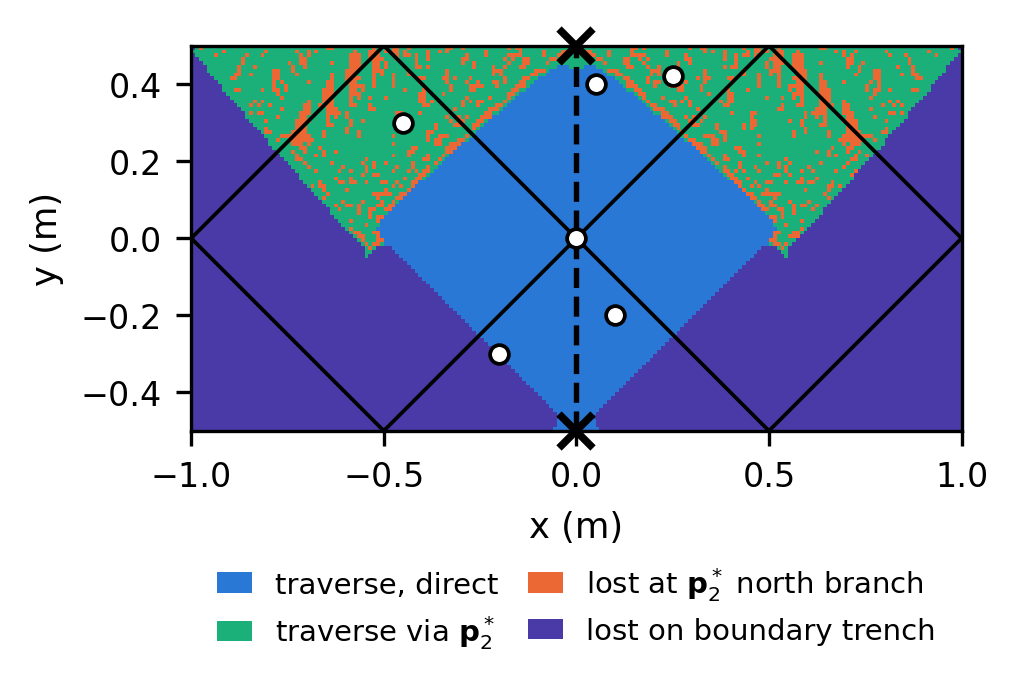
\includegraphics[width=0.34\textwidth]{figures/basin_map.png}
    \caption{Zero-noise, heading-0 outcome of the $D$ tracker from
    every cell of a $200 \times 100$ start grid: direct traverse to
    $\mathbf{p}^*_1$ (26.9\%), traverse via the top wall and
    $\mathbf{p}^*_2$ (20.5\%), loss at the $\mathbf{p}^*_2$ north
    branch (5.6\%), and loss on a boundary trench that exits the
    domain (47.1\%). Okubo-Weiss diamonds ($D = 0$) outlined, separatrix
    dashed, saddles marked $\times$, the six clean-run starts of
    Fig.~\ref{fig:sep_trajectories} marked $\circ$. No start parks at a
    gyre core: the basin is the watershed of the $\hat{D}$ descent, not
    the Okubo-Weiss partition.}
    \label{fig:basin_map}
\end{figure}

No start parks at a gyre core: descent of $\hat{D}$ from the
rotation-dominated interiors reaches the trench network within the
500-step horizon in all 20\,000 runs, so the basin boundary is not the
Okubo-Weiss partition. The map is instead the watershed of the descent
composited with the flow direction on the acquired branch: a central
diamond of direct traverses (26.9\%), an upper region that rides the
top wall to $\mathbf{p}^*_2$ and continues to $\mathbf{p}^*_1$
(20.5\%), interleaved with north-branch losses at the $\mathbf{p}^*_2$
junction (5.6\%), and lower and outer watersheds whose boundary-trench
rides leave the domain without reaching $\mathbf{p}^*_1$
($47.1\%_{\text{grid loss}}$), since the walls are also valley lines
of $D$ and the bottom wall carries flow away from $\mathbf{p}^*_1$. The
grid's own success rate, direct plus top-wall arrivals, is
$26.9\% + 20.5\% = 47.4\%$. Under uniform random starts and headings
over the interior box, a separate Monte Carlo trial gives
$47.1\%_{\text{random}}$ of $n = 10{,}000$ trials reaching
$\mathbf{p}^*_1$ at zero noise: the same quantity, arrival at
$\mathbf{p}^*_1$, measured two independent ways, a deterministic
zero-noise grid and a randomly seeded trial, agreeing to within
sampling noise. That agreement is a consistency check on the basin
map, not a coincidence; $47.1\%_{\text{grid loss}}$ matching
$47.1\%_{\text{random}}$'s digits is the separate, genuine coincidence,
a different quantity entirely (loss on the grid, not success). Prior
adaptive-navigation primitives
\cite{27}, \cite{28} report local convergence without basin estimates.

\section{Conclusion and Future Work}
\label{sec:conclusion}
\label{sec:future}

This paper presented one cooperative estimator and two trackers built
on it. A six-robot formation, proved minimal for the unconstrained
quadratic model, recovers the local
quadratic model of a planar flow from a single synchronous sample, and
with it both terms of the splitting identity $D = \omega^2/4 - s_1^2$,
with closed-form, heading-isotropic noise gains verified to $0.3\%$.
The $D$ tracker rides the connected trench network of $D$ on a modified
Newton step, with a Lyapunov certificate and a network-traversal
theorem whose terminal-capture case is one threshold away. The $s_1$
tracker rides the same network from the strain term alone, with a
capture test built only from the objective gradient where the $D$
tracker's own capture test is known to misfire, and its frame
equivariance was demonstrated in closed loop rather than asserted: the
same material curve in either observer frame (gap 0.025), where the $D$
tracker follows a frame artifact (gap 1.219). Monte Carlo sweeps placed
the $D$ tracker's failure cliff exactly at the estimator's
gradient-reliability threshold, so the estimator, not the control law,
sets its noise ceiling; the $s_1$ tracker's own noise ceiling is set
one level earlier by a different mechanism, the reliability of the
one-time flow-seeded tangent sign rather than the estimator's gradient
accuracy. On
real Santa Barbara Channel currents the $D$ tracker followed a coherent
ridge for 28 hours to a consistent landfall reproduced by 84 of 100
nearby starts, and the $s_1$ tracker converged to and held a stable
local trench loop through the same 28-h record, within 1.4~km of
offline ground truth. Every capability rests on the same premise: a
team that can sense second-order structure locally does not need the
map.

Four extensions are direct. A time-derivative correction term,
analyzed against the analytic $\varepsilon > 0$ double gyre, would
extend the stability results to time-varying fields with a quantified
bound. Online formation reshaping would protect the conditioning of
$\boldsymbol{\Phi}$. Hardware deployment on the Decabot testbed would
close the loop on physical robots. And extension to three dimensions
raises the estimation stakes: ten coefficients per component, so ten
robots, or a reduced-order estimator.

\appendices

\section{Proofs}
\label{app:proofs}

This appendix collects the proofs. The formal statements of
Proposition~\ref{prop:minimality} (minimality), Proposition~\ref{prop:conic}
(conic criterion), Corollary~\ref{cor:pentagon} (pentagon plus center), and
Remark~\ref{rem:minimality_priors} (minimality and structural priors) are
in Section~\ref{sec:estimation}, restated here only where their proofs
need them.

\begin{IEEEproof}[Proof of Proposition~\ref{prop:minimality}]
With $N < 6$, $\boldsymbol{\Phi} \in \mathbb{R}^{N \times 6}$ has a
nontrivial null space, so $\boldsymbol{\theta}_u$ and
$\boldsymbol{\theta}_u + \boldsymbol{\theta}_0$ with
$\boldsymbol{\Phi}\boldsymbol{\theta}_0 = \mathbf{0}$,
$\boldsymbol{\theta}_0 \neq \mathbf{0}$, generate identical
measurements: no estimator can select between them. With $N = 6$,
(\ref{eq:solve}) is uniquely solvable iff $\det(\boldsymbol{\Phi})
\neq 0$.
\end{IEEEproof}

\begin{IEEEproof}[Proof of Proposition~\ref{prop:conic}]
$\boldsymbol{\Phi}$ is singular iff its columns are linearly dependent,
iff there is a nonzero coefficient vector $\mathbf{c}$ with
$\boldsymbol{\phi}(\tilde{\mathbf{p}}_i)^\top \mathbf{c} = 0$ for all
$i$. The function $q = \boldsymbol{\phi}^\top \mathbf{c}$ is precisely a
nonzero polynomial of degree at most two vanishing at all six points.
\end{IEEEproof}

\begin{IEEEproof}[Proof of Corollary~\ref{cor:pentagon}]
The five vertices are in general position, so they determine a unique
conic, their circumscribed circle, which misses the center: no conic
passes through all six points, and Proposition~\ref{prop:conic}
applies.
\end{IEEEproof}

\begin{IEEEproof}[Proof of Lemma~\ref{lem:gains}]
The value coefficient is exact: every basis function except the constant
vanishes at the origin, so interpolation forces $\hat{u}_0$ to equal the
center robot's reading, giving unit gain. The remaining rows follow from
direct inversion of $\boldsymbol{\Phi}$ using the fifth roots of unity;
the row norms reduce to the stated constants, and repeating the
computation with an arbitrary ring phase leaves them unchanged. The
error covariance of the estimated gradient is in fact isotropic,
$\tfrac{4}{10}\sigma_{uv}^2\,\rho^{-2}\mathbf{I}$, for every heading.
\end{IEEEproof}

\begin{IEEEproof}[Proof of Theorem~\ref{thm:attract}]
Since $\nabla V_A = \mathbf{H}_D \mathbf{g}$,
$\dot{V}_A = \mathbf{g}^\top \mathbf{H}_D \boldsymbol{\delta}
= -\sum_k v_{\max} \tanh(z_k/v_{\max})\,
\mathbf{g}^\top \mathbf{H}_D \mathbf{w}_k
= -\sum_k v_{\max} \tanh(z_k/v_{\max})\,\lambda_k
(\mathbf{w}_k^\top\mathbf{g})$, and $\lambda_k(\mathbf{w}_k^\top
\mathbf{g}) = \lambda_k^2 z_k$, giving (\ref{eq:VA_dot}); each summand
is nonnegative because $z\tanh z \geq 0$. Equality requires $z_1 = z_2 =
0$, that is $\mathbf{g} = \mathbf{0}$. Convergence to the critical set
follows from the invariance principle. Near an isolated critical point
$|z_k| \ll v_{\max}$, the saturation is inactive at first order,
$\boldsymbol{\delta} \approx -\mathbf{H}_D^{-1}\mathbf{g} \approx
-(\mathbf{p}_c - \mathbf{p}^\star_D)$, a unit-rate linear contraction.
\end{IEEEproof}

\begin{lemma}[Common transverse contraction]
\label{lem:transverse}
Under Assumption~\ref{ass:trench}(i), in every mode of the $D$ tracker
the transverse coordinate obeys (\ref{eq:n_dynamics}): $|n|$ decreases
strictly for $n \neq 0$, the tube $T_w$ is forward invariant, and
$n \to 0$ exponentially once $|n| \leq v_{\max}$, unaffected by
arbitrary switching among the modes.
\end{lemma}

\begin{IEEEproof}
By (\ref{eq:normal_form}) the Hessian is diagonal in
$(\hat{\mathbf{e}}_\parallel, \hat{\mathbf{e}}_\perp)$ with
transverse eigenvalue $\lambda_\perp > 0$, and the transverse gradient
component is $\lambda_\perp n$. The $\hat{\mathbf{e}}_\perp$
component of the attract, slide, and flow steps (the transverse
eigenvalue is positive, so signed and magnitude denominators agree) is
built from the same argument $-\lambda_\perp n / \lambda_\perp =
-n$,\footnote{For the double gyre itself the normal form holds to
second order rather than exactly: the exact transverse gradient and
curvature give the Newton argument $-\tan(2\pi n)/(2\pi)$ in place of
$-n$, which has the sign of $n$ and magnitude at least $|n|$ for
$|n| < 1/4$, so the resulting contraction is at least as fast as
(\ref{eq:n_dynamics}) and every conclusion that follows is
unchanged.} saturation gives (\ref{eq:n_dynamics}). The right side is negative for $n > 0$ and
positive for $n < 0$, so $V_\perp = \tfrac{1}{2}n^2$ is a common
Lyapunov function for the switched system; for $|n| \leq v_{\max}$,
$\tanh(n/v_{\max}) \geq n \tanh(1)/v_{\max}$ yields $\dot{V}_\perp \leq
-2\tanh(1) V_\perp$.
\end{IEEEproof}

\begin{lemma}[Flow-consistent progress]
\label{lem:progress}
Under Assumption~\ref{ass:trench}, on $\Gamma$ (after the transient of
Lemma~\ref{lem:transverse}) the tangential velocity $\dot{\ell}$
satisfies, in every mode, $\dot{\ell}\,(\mathbf{v}^\top
\hat{\mathbf{e}}_\parallel) \geq 0$: the team never moves against the
ambient flow along the trench. Moreover $|\dot{\ell}| \geq m > 0$ outside
the $r_0$ balls, with
\begin{equation}
    m = \min\Bigl\{
    v_{\max}\tanh\!\bigl(\tfrac{f_{\min}}{v_{\max}}\bigr),\;
    v_{\max}\tanh\!\bigl(\tfrac{m_h}
    {\bar{\lambda}_\parallel v_{\max}}\bigr)
    \Bigr\},
    \label{eq:progress_rate}
\end{equation}
where $\bar{\lambda}_\parallel$ bounds $|\lambda_1|$ on the tube.
\end{lemma}

\begin{IEEEproof}
In every mode the tangential sign agrees with the flow and the
magnitude is bounded below by (\ref{eq:progress_rate}):
\begin{center}
\footnotesize
\begin{tabular}{@{}p{0.16\linewidth}p{0.34\linewidth}p{0.42\linewidth}@{}}
\hline
\textbf{Mode} & \textbf{Tangential command} & \textbf{Why it tracks the flow} \\
\hline
FLOW &
$v_{\max}\tanh\!\bigl(\frac{\mathbf{f}^\top\mathbf{w}_1}{v_{\max}}\bigr)$
along $\mathbf{w}_1$ &
Product form: a nonnegative multiple of the flow's own tangential
component; covers the crest by Assumption~\ref{ass:trench}(ii). \\
SLIDE (off-band) &
$v_{\max}\tanh\!\bigl(\frac{|h'|}{|\lambda_1|v_{\max}}\bigr)$
along descent &
Selected precisely when the flow agrees with the descent direction
$-\mathrm{sign}(h')\hat{\mathbf{e}}_\parallel$. \\
ATTRACT (off-band) &
$-h'/\lambda_1$ ($\lambda_1 < 0$), along ascent, same magnitude &
Selected when the flow opposes descent, so ascent is the flow
direction instead. \\
Attract fallback &
Descends toward the well &
The well's stable-manifold endpoint is the local flow direction. \\
\hline
\end{tabular}
\end{center}
\end{IEEEproof}

\begin{IEEEproof}[Proof of Theorem~\ref{thm:separatrix}]
(i) is Lemma~\ref{lem:transverse}. (ii): by Lemma~\ref{lem:progress},
$\ell(t)$ is monotone in the flow direction with rate at least $m$ outside
the $r_0$ balls, and mode switches cannot reverse it, so the ball is
reached in time at most $L_\Gamma/m$. Capture (iii): inside the ball,
$\mathbf{H}_D \succ 0$, the selector is in its attract fallback, and
Theorem~\ref{thm:attract} gives local exponential convergence to the
well, which coincides with the flow saddle $\mathbf{p}^*$. Continuation:
if the fallback test fails to trigger despite $\mathbf{H}_D \succ 0$
holding for the true field, the selector instead falls through to
Lemma~\ref{lem:progress}'s flow or descent case on whichever of the two
crossing segments the flow direction and sign convention of
$\hat{\mathbf{g}}$ select, and (i)-(ii) apply unchanged with $\Gamma$
relabeled.
\end{IEEEproof}

\begin{IEEEproof}[Proof of Proposition~\ref{prop:equivariance}]
$\mathbf{S}' = \mathbf{Q}\mathbf{S}\mathbf{Q}^\top$, so $s_1' = s_1$,
$r' = r$, $\mathbf{e}_k' = \mathbf{Q}\mathbf{e}_k$, and $\nabla' s_1' =
\mathbf{Q}\nabla s_1$ (the gradient of an invariant scalar co-rotates).
The branch conditions are scalar thresholds on the invariants $r$,
$\hat{s}_1$, and $\lVert\nabla\hat{s}_1\rVert$ (the banded and captured
flags), so each branch fires identically in both frames. The tangent
selection (\ref{eq:d1d2})--(\ref{eq:tangent_select}) uses only the
invariant inner products $\hat{d}_k' = \lvert\nabla' s_1'^\top
\mathbf{e}_k'\rvert = \lvert\nabla s_1^\top \mathbf{e}_k\rvert =
\hat{d}_k$, so the same eigenvector is selected in both frames; its
sign is fixed by $\mathrm{sign}(\mathbf{t}_{\text{ref}}'^\top
\mathbf{t}_{\text{raw}}')$ with $\mathbf{t}_{\text{ref}}' = \mathbf{Q}
\mathbf{t}_{\text{prev}}$ once a previous tangent exists, by induction,
so from the second tracking step onward the inner product is invariant
and $\hat{\mathbf{t}}' = \mathbf{Q}\hat{\mathbf{t}}$. PARK, CAPTURE, and
the transverse channel (\ref{eq:oecs_perp}) apply the invariant gradient
along $\hat{\mathbf{n}}' = \mathbf{Q}\hat{\mathbf{n}}$ (whichever
eigenvector $\hat{\mathbf{t}}$ did not select, itself co-rotating by the
same argument), and the tangential channel commands
$v_{\max}\tanh(1)\hat{\mathbf{t}}'$; all three output the rotated
command $\mathbf{Q}\boldsymbol{\delta}$ from the second tracking step
on. Two inputs are not exactly covariant (ACQUIRE, whose observer-axis
saturation still descends the invariant $\hat{s}_1$ in either frame,
per the body statement above), both confined to a single
instant: CROSS's direct use of the flow $\mathbf{f}$, reached only if
$r < r_{\text{band}}$ on the first tracking step with no
$\mathbf{t}_{\text{prev}}$ established, and the sign reference on
TRACK's own first invocation whenever CROSS is not reached, where
$\mathbf{t}_{\text{ref}} = \mathbf{f}$ in the absence of a previous
tangent. Under a time-dependent $\mathbf{Q}(t)$ the measured flow in the
rotating frame carries the transport term
$\dot{\mathbf{Q}}\mathbf{Q}^\top\mathbf{p}'$, which has no counterpart
in the inertial frame, so at this one instant the resolved sign is not
guaranteed to agree between frames; thereafter, by the induction above,
it is carried forward by continuity alone and the closed loop is
covariant for the remainder of the run. This is the same single-instant
caveat the $D$ tracker's own ride mode carries for its own tangent seed.
\end{IEEEproof}

\begin{thebibliography}{99}

\bibitem{1} J. Cortés and M. Egerstedt, "Coordinated control of multi-robot
systems: A survey," \textit{SICE Journal of Control, Measurement, and
System Integration}, vol. 10, no. 6, pp. 495--503, 2017.

\bibitem{2} J. Das et al., "Coordinated sampling of dynamic oceanographic
features with underwater vehicles and drifters," \textit{The International
Journal of Robotics Research}, vol. 31, no. 5, pp. 626--646, 2012.

\bibitem{3} S. McCammon et al., "Ocean front detection and tracking using a
team of heterogeneous marine vehicles," \textit{Journal of Field Robotics},
vol. 38, no. 6, pp. 854--881, 2021.

\bibitem{4} S. R. Ramp et al., "Preparing to predict: the second autonomous
ocean sampling network (AOSN-II) experiment in the Monterey Bay,"
\textit{Deep Sea Research Part II: Topical Studies in Oceanography}, vol. 56,
no. 3-5, pp. 68--86, 2009.

\bibitem{5} C. Dong et al., "Oceanic mesoscale eddies," \textit{Ocean-Land-
Atmosphere Research}, vol. 4, p. 0081, 2025.

\bibitem{6} G. Haller and G. Yuan, "Lagrangian coherent structures and mixing
in two-dimensional turbulence," \textit{Physica D: Nonlinear Phenomena},
vol. 147, no. 3-4, pp. 352--370, 2000.

\bibitem{7} T. Peacock and G. Haller, "Lagrangian coherent structures: The
hidden skeleton of fluid flows," \textit{Physics Today}, vol. 66, no. 2,
pp. 41--47, 2013.

\bibitem{8} S. C. Shadden, F. Lekien, and J. E. Marsden, "Definition and
properties of Lagrangian coherent structures from finite-time Lyapunov
exponents in two-dimensional aperiodic flows," \textit{Physica D}, vol. 212,
no. 3-4, pp. 271--304, 2005.

\bibitem{9} M. Michini, M. A. Hsieh, E. Forgoston, and I. B. Schwartz,
"Robotic tracking of coherent structures in flows," \textit{IEEE Transactions
on Robotics}, vol. 30, no. 3, pp. 593--603, 2014.

\bibitem{10} M. Michini, H. Rastgoftar, M. A. Hsieh, and S. Jayasuriya,
"Distributed formation control for collaborative tracking of manifolds in
flows," in \textit{Proc. American Control Conference}, pp. 3874--3880, 2014.

\bibitem{11} M. Michini, M. A. Hsieh, E. Forgoston, and I. B. Schwartz,
"Experimental validation of robotic manifold tracking in gyre-like flows,"
in \textit{Proc. IEEE/RSJ International Conference on Intelligent Robots
and Systems (IROS)}, pp. 2306--2311, 2014.

\bibitem{12} G. Knizhnik, P. Li, X. Yu, and M. A. Hsieh, "Flow-based control
of marine robots in gyre-like environments," in \textit{Proc. 2022 Int. Conf.
on Robotics and Automation (ICRA)}, pp. 3047--3053, 2022.

\bibitem{13} D. Kularatne and M. A. Hsieh, "Tracking attracting manifolds in
flows," \textit{Autonomous Robots}, vol. 41, no. 8, pp. 1575--1588, 2017.

\bibitem{14} C. Waight and C. A. Kitts, "Adaptive navigation of multirobot
systems to critical points in 2D vector fields," submitted for publication.

\bibitem{15} L. Briñón-Arranz, A. Renzaglia, and L. Schenato, "Multirobot
symmetric formations for gradient and Hessian estimation with application to
source seeking," \textit{IEEE Transactions on Robotics}, vol. 35, no. 3,
pp. 782--789, 2019.

\bibitem{16} G. Haller, "Lagrangian coherent structures," \textit{Annual
Review of Fluid Mechanics}, vol. 47, pp. 137--162, 2015.

\bibitem{17} M. Serra and G. Haller, "Objective Eulerian coherent
structures," \textit{Chaos: An Interdisciplinary Journal of Nonlinear
Science}, vol. 26, no. 5, p. 053110, 2016.

\bibitem{18} P. J. Nolan, M. Serra, and S. D. Ross, "Finite-time Lyapunov
exponents in the instantaneous limit and material transport,"
\textit{Nonlinear Dynamics}, vol. 100, no. 4, pp. 3825--3852, 2020.

\bibitem{19} T. D. Harms, S. T. M. Dawson, and B. J. McKeon, "Lagrangian
gradient regression for the detection of coherent structures from sparse
trajectory data," \textit{Royal Society Open Science}, vol. 11, no. 9,
p. 240586, 2024.

\bibitem{20} G. Haller, "Dynamic rotation and stretch tensors from a
dynamic polar decomposition," \textit{Journal of the Mechanics and Physics
of Solids}, vol. 86, pp. 70--93, 2016.

\bibitem{21} A. Okubo, "Horizontal dispersion of floatable particles in the
vicinity of velocity singularities such as convergences," \textit{Deep-Sea
Research}, vol. 17, no. 3, pp. 445--454, 1970.

\bibitem{22} J. Weiss, "The dynamics of enstrophy transfer in two-dimensional
hydrodynamics," \textit{Physica D: Nonlinear Phenomena}, vol. 48, no. 2-3,
pp. 273--294, 1991.

\bibitem{23} J. C. R. Hunt, A. A. Wray, and P. Moin, "Eddies, streams, and
convergence zones in turbulent flows," in \textit{Proc. Summer Program,
Center for Turbulence Research}, Rep. CTR-S88, pp. 193--208, 1988.

\bibitem{24} B.-L. Hua and P. Klein, "An exact criterion for the stirring
properties of nearly two-dimensional turbulence," \textit{Physica D}, vol. 113,
no. 1, pp. 98--110, 1998.

\bibitem{25} R. Cooper et al., "Initial study of multirobot adaptive
navigation for exploring environmental vector fields," in \textit{Proc.
IEEE Aerospace Conference}, 2019.

\bibitem{26} P. Ögren, E. Fiorelli, and N. E. Leonard, "Cooperative control
of mobile sensor networks: Adaptive gradient climbing in a distributed
environment," \textit{IEEE Transactions on Automatic Control}, vol. 49, no. 8,
pp. 1292--1302, 2004.

\bibitem{27} R. T. McDonald, C. A. Kitts, and M. A. Neumann, "Navigation of
scalar fronts with multirobot clusters in simulation and experiment,"
\textit{IEEE Systems Journal}, vol. 14, no. 3, pp. 3755--3766, 2020.

\bibitem{28} C. A. Kitts, R. T. McDonald, and M. A. Neumann, "Adaptive
navigation control primitives for multirobot clusters: Extrema finding,
contour following, ridge/trench following, and saddle point station keeping,"
\textit{IEEE Access}, vol. 6, pp. 17625--17642, 2018.

\bibitem{29} R. T. McDonald, C. A. Kitts, and M. A. Neumann, "Experimental
implementation and verification of scalar field ridge, trench, and saddle
point maneuvers using multirobot adaptive navigation," \textit{IEEE Access},
vol. 7, pp. 62950--62961, 2019.

\bibitem{30} C. A. Kitts and I. Mas, "Cluster space specification and control
of mobile multirobot systems," \textit{IEEE/ASME Transactions on Mechatronics},
vol. 14, no. 2, pp. 207--218, 2009.

\bibitem{31} T. Adamek, C. A. Kitts, and I. Mas, "Gradient-based cluster space
navigation for autonomous surface vessels," \textit{IEEE/ASME Transactions on
Mechatronics}, vol. 20, no. 2, pp. 506--518, 2014.

\bibitem{32} S. Tomer et al., "A low-cost indoor testbed for multirobot
adaptive navigation research," in \textit{Proc. IEEE Aerospace Conference},
pp. 1--12, 2018.

\bibitem{33} C. Waight and C. Kitts, "A functional indoor testbed for
multirobot adaptive navigation in vector field environments," in
\textit{Proc. ASME Int. Design Engineering Technical Conf. and Computers
and Information in Engineering Conf.}, vol. 89251, 2025.

\bibitem{35} Y. N. Dauphin, R. Pascanu, C. Gulcehre, K. Cho, S. Ganguli,
and Y. Bengio, "Identifying and attacking the saddle point problem in
high-dimensional non-convex optimization," in \textit{Advances in Neural
Information Processing Systems}, vol. 27, pp. 2933--2941, 2014.

\bibitem{36} M. Serra, P. Sathe, I. Rypina, A. Kirincich, S. D. Ross,
P. Lermusiaux, A. Allen, T. Peacock, and G. Haller, "Search and rescue
at sea aided by hidden flow structures," \textit{Nature Communications},
vol. 11, no. 1, p. 2525, 2020.

\bibitem{37} W. Yao, H. G. de Marina, B. Lin, and M. Cao,
"Singularity-free guiding vector field for robot navigation,"
\textit{IEEE Trans. Robot.}, vol. 37, no. 4, pp. 1206--1221, 2021.

\bibitem{38} T. Liddy and T.-F. Lu, "Obstacle avoidance using complex
vector fields," in \textit{Proc. Australasian Conf. Robotics and
Automation (ACRA)}, 2008.

\end{thebibliography}

\end{document}
